% !TEX TS-program = xelatex
% !BIB program = bibtex
% !TEX encoding = UTF-8 Unicode

\documentclass[
  oneside,				% use oneside to prevent empty page with numbering
  openright,
  degree    = master,               % degree = master | doctor
  language  = english,              % language = chinese | english
  fontset   = template,             % fontset = default | template | system | overleaf
  watermark = false,                 % watermark = true | false
  doi       = false,                 % doi = true | false
]{ntuthesis}

% 注意封面不會產生浮水印(即使watermark = true)!但會有DOI。依學校規定,封面需要有浮水印,建議先生成無浮水印的檔案,在使用pdf編輯軟體加入浮水印。


% !TeX root = ./main.tex

% --------------------------------------------------
% 資訊設定(Information Configs)
% --------------------------------------------------

\ntusetup{
  university*   = {National Taiwan University},
  university    = {國立臺灣大學},
  college       = {生命科學院},
  college*      = {College of Life Science},
  institute     = {生態學與演化生物學研究所},
  institute*    = {Institute of Ecology and Evolutionary Biology},
  title         = {整合不同分析方法來量化關聯群落背後的生態機制},
  title*        = {Disentangling ecological processes underlying the metacommunity by integrating several analytical methods},
  author        = {黃敬麟},
  author*       = {Ching-Lin Huang},
  ID            = {R09b44010},
  advisor       = {澤大衛},
  advisor*      = {David Zelený,},	   % note "," after names
  date          = {2023-1-16},         % 若註解掉,則預設為當天
  oral-date     = {2023-1-16},         % 若註解掉,則預設為當天
  DOI           = {10.6342/NTU202300163},
  keywords      = {群落組成, 觀察資料, 福山森林動態樣區, 機制群落模型, 隨機森林, 模擬},
  keywords*     = {community assembly, empirical data, Fushan Forest Dynamics Plot, process-based model, random forest, simulation},
}

% --------------------------------------------------
% 加載套件(Include Packages)
% --------------------------------------------------

\usepackage{natbib}     				% 參考文獻
\usepackage{hyperref} 					% hyperlink for sections
\usepackage{amsmath, amsthm, amssymb}   % 數學環境
%\usepackage{ulem, CJKulem}             % 下劃線、雙下劃線與波浪紋效果
\usepackage{booktabs}                   % 改善表格設置
\usepackage{multirow}                   % 合併儲存格
\usepackage{diagbox}                    % 插入表格反斜線
\usepackage{array}                      % 調整表格高度
\usepackage{longtable}                  % 支援跨頁長表格
\usepackage{paralist}                   % 列表環境
\usepackage{afterpage}					% continue longtable
\usepackage{xurl}						% auto-change line for url
\usepackage{pdfpages}					% insert pdf

% set of chapters

% --------------------------------------------------
% 套件設定(Packages Settings)
% --------------------------------------------------
\counterwithout{figure}{chapter} 		% continuous label for figures
\counterwithout{table}{chapter} 		% continuous lael for tables


\begin{document}

% 封面與口試審定
% Cover and Verification Letter
\makecover                          % 論文封面(Cover)

\pagenumbering{roman}			    % numbering in roman before main text
%\makeverification                 % 口試委員審定書(Verification Letter)
% Insert pdf file of signed verification letter
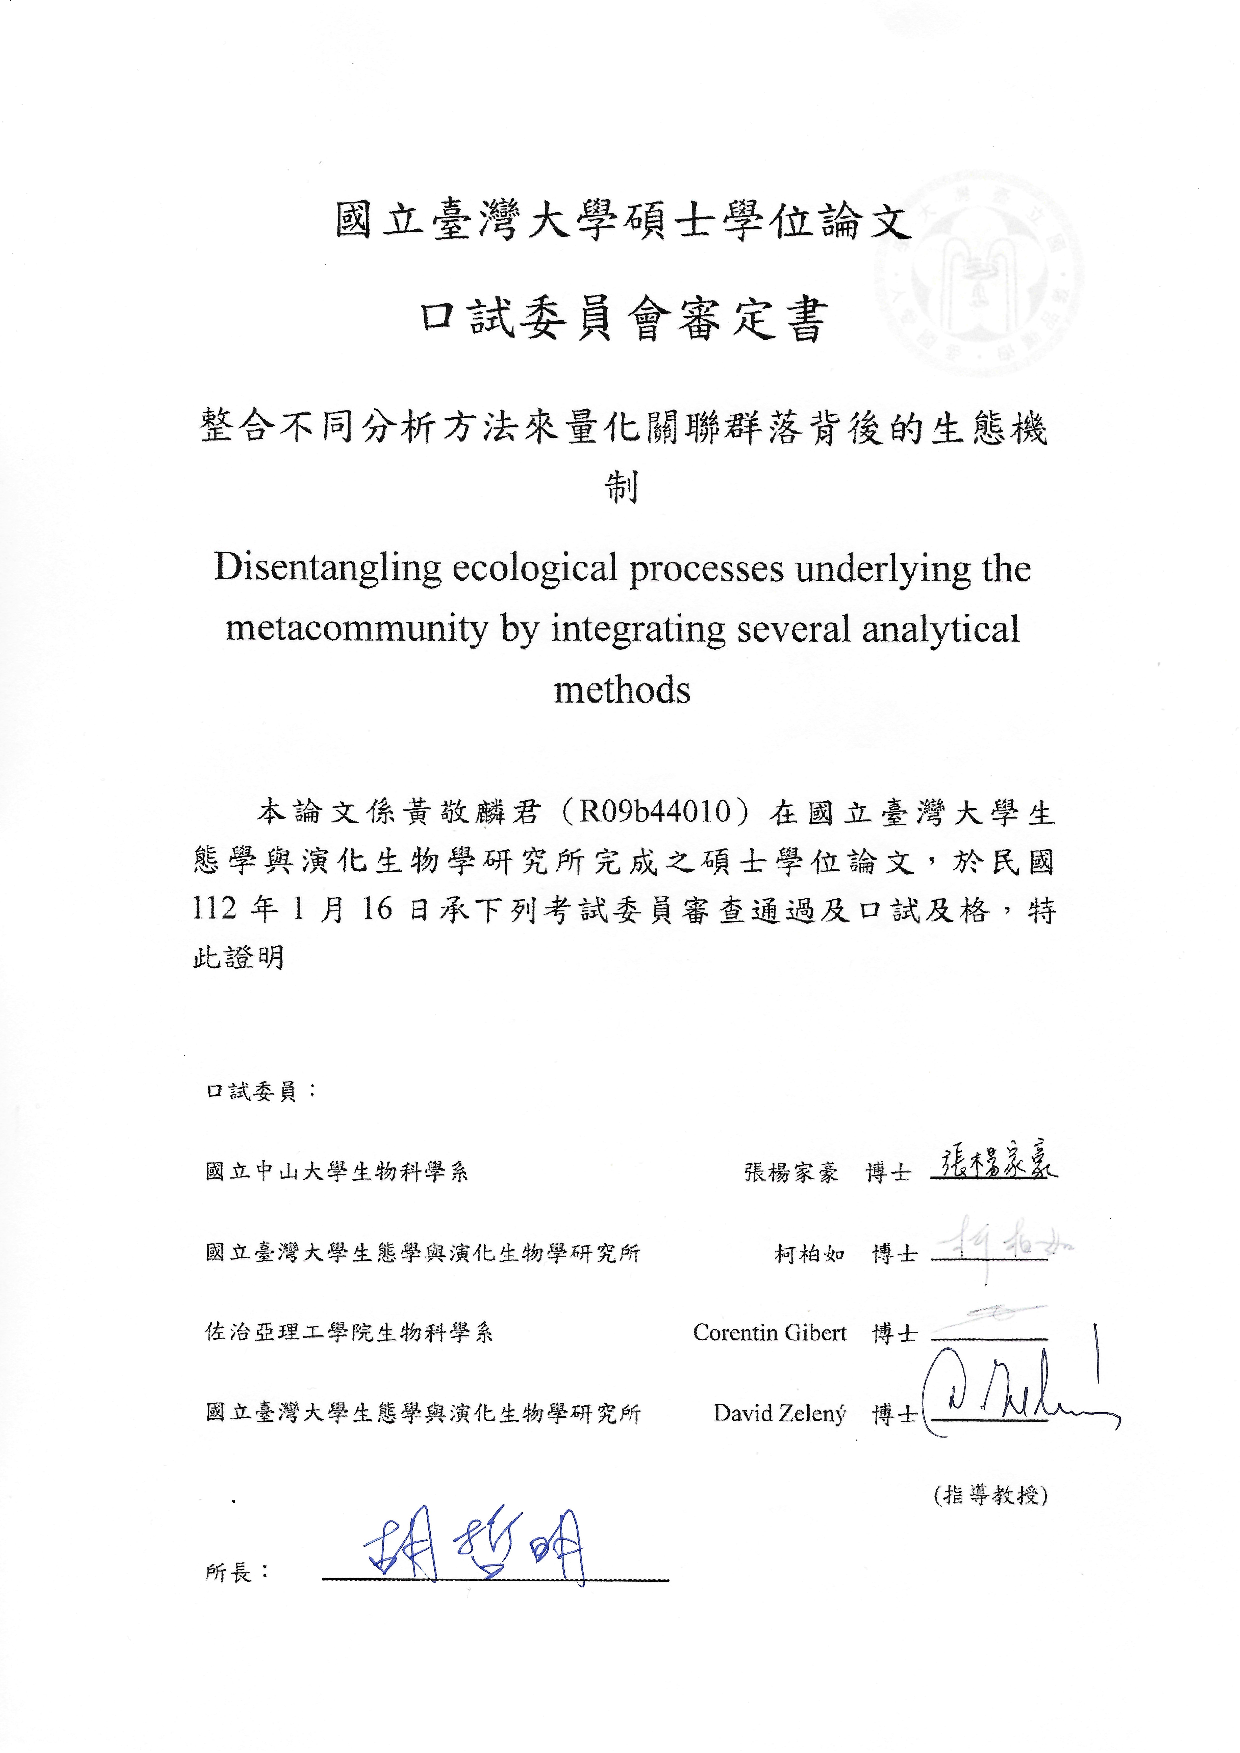
\includepdf[pages=-, pagecommand={\thispagestyle{plain}
\addcontentsline{toc}{chapter}{Verification Letter from the Oral Examination Committee}}]{front/Verification_Letter.pdf}



% 致謝與論文摘要
% Acknowledgement and Abstract
% !TeX root = ../main.tex

\begin{acknowledgement}
	不知不覺,已經步入生態學的世界四年了。自從在大三的時候修了五木老師的樹木學,開始燃起我對於自然世界的興趣,也促使我去參加了2019年的福山森林動態樣區的每木調查。在福山跟家豪聊過之後,我才發現生態的研究是有用到蠻多數學的,讓我覺得自己的數學背景並不會讓我在這個領域太過突兀。調查結束之後,在台大找到了大衛的研究室,這才真正的開始我在生態領域中的旅程。
	
	真的非常感謝我的指導教授David,每次都花很多心力和腦力在跟我討論我的研究方向和分析結果。這兩年半來,他帶我認識生態研究中的許多不同面相,教我如何嚴謹的做研究、思考問題和挖掘每個問題背後的價值。在分析資料的部分,我借用研究室的電腦,好讓我跑分析的時候能有足夠的記憶體來處理龐大的資料量。在撰寫論文的時候,David也很用心的給我建議,並跟我討論要怎麼寫才能讓句子變得精準但又好懂。David同時也是一位很棒的人生導師,他在我面對人生的無常的時候安慰我,也告訴我要去好好接納和感受自己的情緒和想法,這些建議始終影響和造就著現在我。同時,我也感謝柯柏如老師和我討論撰寫論文的大方向。感謝張楊家豪老師讓我使用福山四年的資料,來演示我的方法。感謝Corentin老師願意接受台美遠距口試,給了我很多發表上的建議。另外也感謝魏碩、宇霈、晟洋、書逸、訓宏、尹舜和其他研究室的夥伴時常在能一起討論生態問題或是吃飯聊聊天,讓研究所的生活不這麼苦悶。感謝柏佑在口試前後幫助我很多在行政上的事。感謝亭羽和其他朋友、家人,在寫論文的時候陪伴我或是給予支持,讓我能順利的度過這個焦慮的時期。
	
	看越多文獻,就越發現在生態領域中有很多不同面向的研究,也有許多未解的問題。這個世界越看越覺得廣大和有趣,期許自己能成為一個站在最前線、探索未知的世界的冒險者。

\end{acknowledgement}       % 致謝(Acknowledgement)
% !TeX root = ../main.tex

\begin{abstract}

關聯群落(metacommunity)由多個群落所組成,並且被四種生態機制所影響:競爭(competition)、環境過濾(environmental filtering)、遷徙(dispersal)和隨機性(stochasticity)。許多方法被用來量化群落組成背後的機制,但僅有少數研究將這些方法整合起來。Guzman等人(2022)整合多種分析方法來量化群落組成背後的機制並使用模擬資料評估其效力。雖然他們的研究整合了多種分析方法,並總結只有結合多種分析方法並應用在完整的關聯群落資料上,才有較高的準確率去量化機制,但他們沒有提出其方法能否應用在實際資料上。本研究討論了Guzman等人(2022)的方法能否應用在實際的生態研究中。我們利用關聯群落模型來產生模擬資料,其模型考慮了非生物和生物間的交互作用以及遷徙等機制。透過調整模型的參數,我們可以改變機制的強度。本研究考慮了三種分析方法:beta-diversity variation partitioning、Stegen方法和dispersal niche continuum index,並利用隨機森林(random forest)將這些分析方法產生的統計量與模擬模型的參數連結起來。根據模擬資料,本研究顯示,越多的分析方法和完整的時間尺度資料被結合起來,估計參數的準確率就會變高。本研究也發現,當資料不完整時,我們對於機制的估計會變得不準確,與Guzman等人(2022)指出的相同。本研究另外展示了Guzman等人(2022)的方法在福山森林動態樣區的應用,發現在福山的物種之間擁有競爭和遷徙之間的權衡(competition-colonization trade-off),並探討在使用其方法時需要考慮的地方。


\end{abstract}

\begin{abstract*}
\noindent
A metacommunity is a set of interconnected communities that incorporate multiple co-occurring species with different abundances. The species composition of a metacommunity is shaped by four main ecological processes: competition, environmental filtering, dispersal and stochasticity. Ecologists have proposed several analytical methods, such as beta-diversity variation partitioning, to quantify the relative importance of ecological processes in shaping metacommunity composition based on information derived from metacommunity composition structure. However, these analytical methods were rarely synthesized. Guzman et al. (2022) integrated multiple analytical methods to estimate the relative importance of ecological processes and evaluated their framework based on the simulated data generated by a process-based simulation model. They concluded that integrating multiple analytical methods and high completeness of the metacommunity across space and time will improve the correctness of the estimation of process-based model parameters. However, the authors did not discuss whether their framework could be applied to observational data. In our study, we reconstructed Guzman et al.'s framework and discussed its application value to the empirical community data. We used the same process-based model as Guzman et al. to generate simulated metacommunity data, incorporating abiotic and biotic interactions, dispersal, and stochasticity. We manipulated the parameters of these four processes to generate metacommunity scenarios with different strengths of underlying processes. We used three analytical methods to calculate summary statistics of the simulated data: 1) beta-diversity variation partitioning, 2) Stegen's framework, and 3) dispersal-niche continuum index (DNCI). We then used the random forest algorithm to estimate the parameters of the process-based model and disentangle different metacommunity scenarios based on the summary statistics. Based on the simulated data, we showed that if the random forest model incorporated the summary statistics derived from more analytical methods and more snapshots of the species composition, it will have better accuracy for estimating the model parameters. We also showed that the incompleteness of the species composition data will decrease the accuracy in estimating the model parameters. On the contrary, the accuracy was not influenced by the choice of the snapshots in the simulation. We also illustrated the application of the trained random forest by analyzing repeated census of woody plant species in the Fushan Forest Dynamics Plot and showed that the community of this forest is based mainly on competition-colonization trade-off. We also discussed what needs to be considered when Guzman et al.'s framework is applied. We conclude that Guzman et al.'s framework based on integrated analytical methods could be successfully applied to observational studies to disentangle the ecological processes shaping observed metacommunity.

\end{abstract*}              % 摘要(Abstract)

% 生成目錄與符號列表
% Contents of Tables and Denotation
\maketableofcontents                % 目錄(Table of Contents)
\makelistoffigures                  % 圖目錄(List of Figures)
\makelistoftables                   % 表目錄(List of Tables)


% 論文內容
% Contents of Thesis
\mainmatter
% !TeX root = ../main.tex

\chapter*{1. Introduction}
\setcounter{chapter}{1}
\addcontentsline{toc}{chapter}{1. Introduction}
\noindent
Diverse ecological processes result in different species composition in the metacommunity across space and time. Ecologists have proposed several analytical methods to estimate the strength of these underlying processes. However, since in natural communities we often do not know the real impact of these processes on the variation of species composition, those analytical methods are difficult to evaluate and compare. One solution may be to draw support from metacommunity simulation models. By using community data which is simulated based on the known strength of ecological processes, we may evaluate whether the implications derived by the analytical methods is accurate or not. In our study, we use simulated datasets to explore the behaviors of multiple analytical methods and study whether they can successfully estimate the strength of the ecological processes underlying the observed metacommunities.

\section{Effects of multiple processes on metacommunity structure}
\noindent
Four high-level ecological processes simultaneously affect the species composition dynamics within a metacommunity. At a local scale, competition and ecological drift are the processes that may determine the local community structure \citep{leibold2004metacommunity}. Competition is a negative species interaction that describes the impact of the population size of a species on the growth rate of itself or the other species. The coexistence of the competing species may result from the differentiation in resource usage or the similarity in fitness (or carrying capacity) of the species \citep{macarthur1967limiting, chesson2000mechanisms}. In contrast, ecological drift is a stochastic process that describes the cause of demographical or environmental stochasticity in the death of an individual or the local extinction of a species within a community \citep{hubbell2011unified}. After an individual dies, the space is released and the surrounding species may have a chance to establish in the newly available space \citep{fukami2015historical}. At the regional scale, environmental filtering and dispersal may play the role in regulating species turnover \citep{leibold2004metacommunity}. The species that can not tolerate given abiotic environmental conditions will be absent from the local community \citep{kraft2015community}. Different dispersal ability of the species may alleviate or facilitate the flow of propagules between local communities \citep{tilman1997community, macarthur1967theory}. These ecological processes may interact with each other and simultaneously drive the species turnover across spatial and temporal scales \citep{thompson2020process}. Metacommunity archetypes describe different perspectives of a metacommunity and focus on the effects of various sets of ecological processes \citep{leibold2004metacommunity, leibold2017metacommunity} (Tab. \ref{tbl:def}). 

Predicting the future dynamics of the metacommunity structure under the pressure of anthropogenic activity and climate change has already become an essential topic in conservation \citep{clark2001ecological, evans2012modelling, chase2020biodiversity}. By studying the relationship between anthropogenic factors and climatic conditions to the strength of ecological processes across metacommunities, the mechanisms underlying the loss of ecosystem services may be disentangled. This may improve the management decisions to optimize ecosystem services \citep{hodgson2019investigating, chase2020biodiversity}. How to estimate the strength of ecological processes underlying the observed metacommunities thereby becomes an urgent question that is related to human welfare.

Process-based modeling is an approach to studying how the ecological processes would affect the species composition of a metacommunity. A process-based model is defined as “a model that characterizes changes in a system's state as explicit functions of the events that drive those state changes” \citep{connolly2017process}. It does not need to be deterministic, but it can also encompass stochastic ecological processes, such as demographic stochasticity and dispersal \citep{connolly2017process}. The parameters in the model may represent the strength of certain ecological processes. By altering the parameters within the process-based model, we may study the effect of the processes on species coexistence \citep{adler2007niche, adler2010coexistence} and the relative abundance of the species \citep{ke2015soil}. Moreover, by fitting the model parameters in the process-based model, the strength of the ecological processes underlying the observed metacommunity may be disentangled. For example, \citet{adler2010coexistence} fitted process-based models by four plant species data from U.S. Sheep Experiment Station and proposed that stabilizing mechanisms are important to maintain the diversity of plant community.


\afterpage{
	\begin{footnotesize}
		\begin{longtable}{p{0.35\textwidth}p{0.6\textwidth}}
			\caption[Definition of the terms used in our study.]{\small
				Definition of the terms used in our study.}
			\label{tbl:def}
			\endfirsthead
			\toprule
			Term & Definition\\
			\midrule
			Species turnover & The changes in species composition across space and time.\\
			Metacommunity & A metacommunity is a set of local communities linked by the dispersal of multiple interacting species \citep{wilson1992complex, leibold2004metacommunity}. In our study, the observed metacommunity is defined as the metacommunity in the field, and the simulated metacommunity is the metacommunity generated by the simulation model.\\
			Ecological process & The force that drives the species turnover across space and time. In the metacommunity ecology framework, four high-level processes are proposed to drive species turnover: competition, ecological drift, environmental filtering and dispersal \citep{leibold2017metacommunity}.\\
			Metacommunity archetypes & Four metacommunity archetypes are the different perspectives to study the species turnover within the metacommunity \citep{leibold2004metacommunity, leibold2017metacommunity}:\\
			\hspace{1em} \textit{Patch dynamics} (PD) & Competition hierarchy and trade-off in competition and colonization ability among species determine the local extinction and colonization of the species and further cause the species turnover within the metacommunity.\\
			\hspace{1em} \textit{Species sorting} (SS) & Species interaction and demographic differences between species, which are associated with the environmental heterogeneity across space and time, are the main drivers of the species turnover within the metacommunity.\\
			\hspace{1em} \textit{Neutral dynamics} (ND) & Species in the metacommunity are demographically similar. Dispersal limitation among local communities and ecological drift caused by the demographic stochasticity within the local patches are the main drivers of species turnover.\\
			\hspace{1em} \textit{Mass effect} (ME) & The species composition is influenced not only by species interactions and demographic differences resulting from environmental heterogeneity, but also by the strong dispersal flow of propagules. The strong dispersal ability of species may prevent the local population of less competitive species from being out-competed and maintain their presence in the community.\\
			Analytical methods & The analytical methods discussed in our study are the statistical approaches that summarize the ecological information based on the ecological community data by multiple summary statistics. The summary statistics may indicate the influence of certain ecological processes on species turnover. For example, beta-diversity variation partitioning is one of the analytical methods that uses constrained ordination to relate species composition with environmental and geographical variables. The variation explained by environmental and geographical variables are the summary statistics of this method.\\
			Process-based simulation models & The process-based approach explicitly models the effect of ecological processes on the state of the system, e.g. population size. The parameters in the process-based model may regulate the strength of the ecological processes. By modifying the model parameters, we may study how species composition would be influenced by the ecological processes.\\
			\bottomrule
		\end{longtable}
	\end{footnotesize}
}

\section{Analytical methods to infer the underlying ecological processes}
\noindent
Ecologists have proposed many analytical methods that aim to identify the presence (or quantify the relative importance) of various ecological processes since the mid of 20th century \citep{macarthur1958population, diamond1975island}. More recently, ecologists starts to integrate multiple types of data, e.g. data about the environmental conditions, functional traits and phylogeny, and propose various analytical methods to summarize the ecological information from the observed metacommunity by multiple summary statistics. These summary statistics serve the purpose to quantify the effect of certain ecological processes on the species turnover or variation in functional traits and phylogeny structure (Fig. \ref{fig:framework}a). 

Null model is one of the approaches that compare the observed community data to the one after randomization \citep{gotelli2006null, gotelli2012statistical}. Randomized data is assumed to represent a metacommunity unaffected by certain underlying processes, which is suggested to be the null hypothesis. If the observed data is considerably different from the randomized one, i.e. the null hypothesis is rejected, then the presence of the processes may be confirmed. Without information on the habitat condition, studying the clustering or over-dispersion of the species composition may disentangle the effect of environmental filtering and competition on species turnover among local communities \citep{diamond1975island, connor1979assembly, chase2011disentangling}. On the other hand, testing the convergence or the divergence of the functional traits and phylogeny composition between communities may also identify whether the observed metacommunity is mainly driven by environmental filtering or competition \citep{mayfield2010opposing, borics2020trait}. The null model approach may also quantify the relative importance of niche and dispersal processes underlying the metacommunity based on species composition and their phylogeny or functional traits \citep{stegen2013quantifying, ford2020functional}, or only based on species composition \citep{gibert2019per, vilmi2021dispersal}. Environmental and geographical data are dispensable for these null model-based analytical methods, which benefits the empiricists to apply these methods in practice. However, it is difficult to benchmark whether the algorithm of randomization correctly diminishes the effect of certain ecological processes. The mismatch between the algorithm and the null hypothesis may result in the wrong type I error rate of the hypothesis testing \citep{molina2020difficulties}.   

Other analytical methods are based on the summary statistics derived from the correlation between different types of data, e.g. canonical analysis and hierarchical joint species distribution approach. By canonical analysis, species composition is regressed on environmental and geographical attributes \citep{borcard1992partialling}, or even functional traits and phylogeny structure within the local communities \citep{sirbu2021variation}. We will refer to this approach as beta-diversity variation partitioning in the following text. The relative importance of environmental filtering and dispersal may be estimated by the amount of compositional variation explained by environmental and geographical data \citep{cottenie2005integrating}. The hierarchical joint species distribution approach uses a hierarchical generalized linear model to relate species composition with environment, traits and phylogeny. In the hierarchical modeling of species community (HMSC) proposed by \citet{ovaskainen2017make}, the random effects of biotic interaction, and spatial and temporal autocorrelation are also considered in the model. The effect of environmental filtering, biotic interaction and random processes on the species turnover may be quantified by the variation partitioning among the explanatory variables in the hierarchical generalized linear model \citep{ovaskainen2017make}.

\begin{figure}
	\centering
	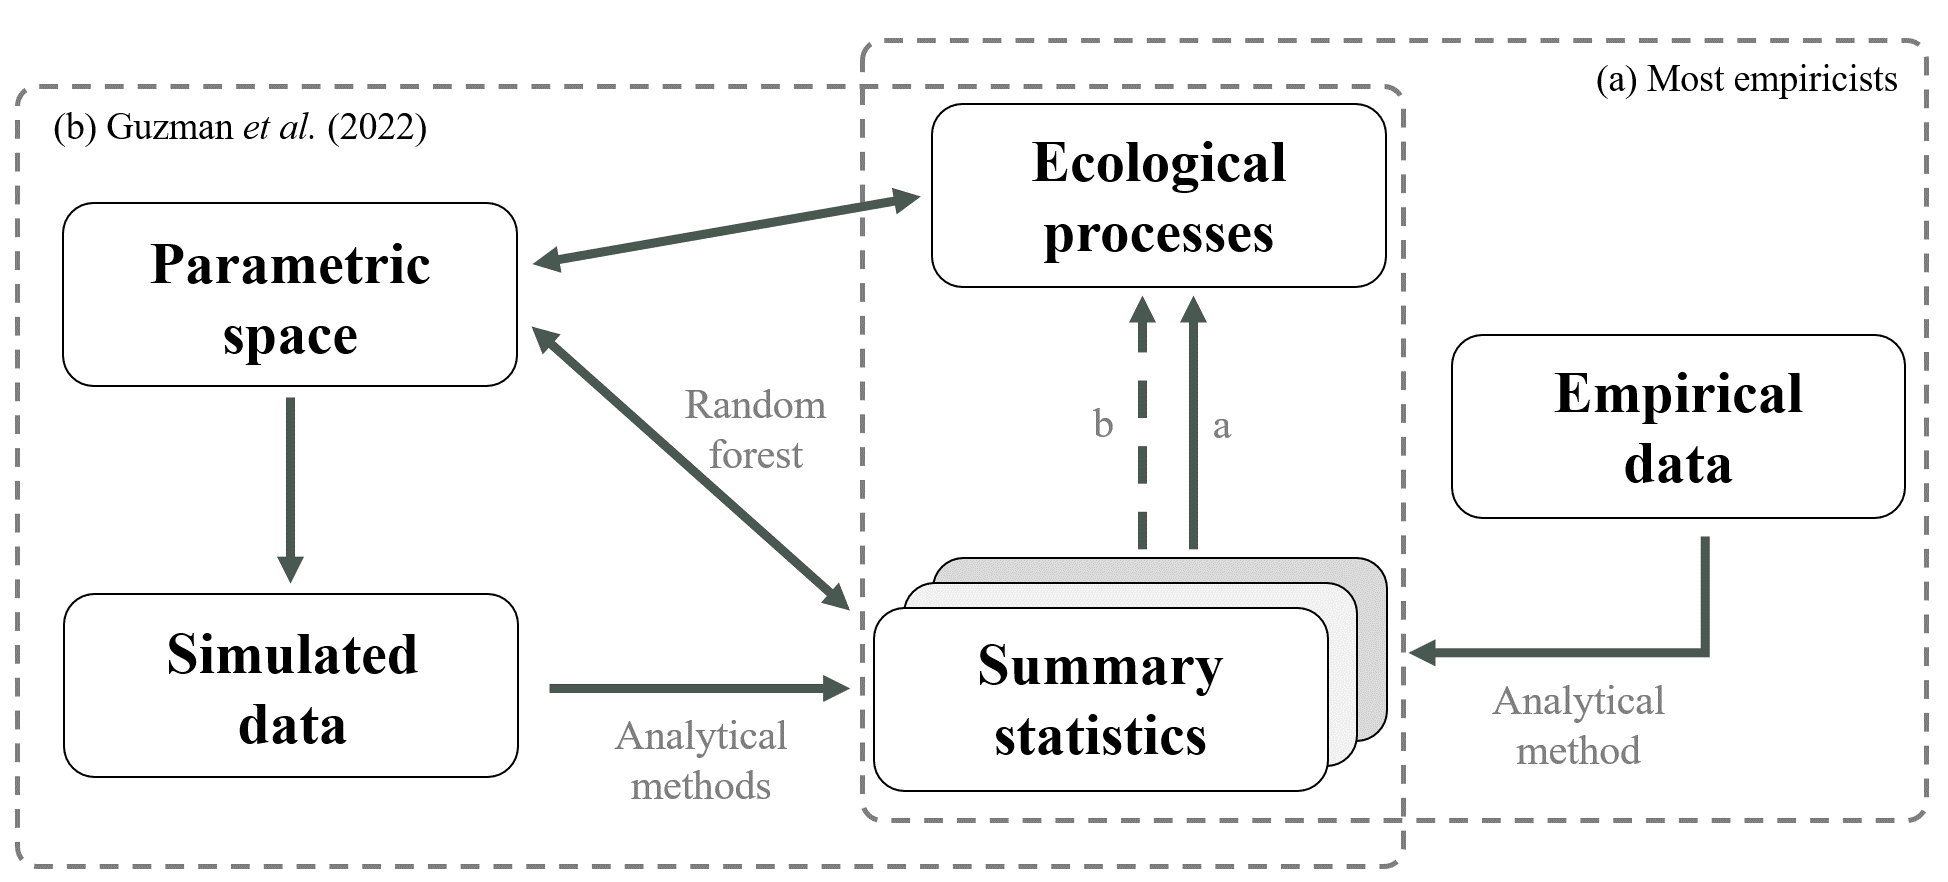
\includegraphics[width=\linewidth]{./figures/ppt/framework.png}
	\caption[Difference between the path most empiricists would take with the path proposed by \citet{guzman2022accounting}.]{\small
		Flow diagram, showing the difference between the path most empiricists would take (box (a) at the right side), compared to the path proposed by \citet{guzman2022accounting} (box (b) at the left side). (a) Most empiricists disentangle the ecological processes underlying the observed metacommunities based on the summary statistics calculated by a single analytical method. For example, beta-diversity is one of the analytical methods to quantify the relative importance of environmental filtering and dispersal on species turnover based on the explained variations in constrained ordination. (b) \citet{guzman2022accounting} extended this process by linking multiple summary statistics derived from different analytical methods to the parametric space of the process-based simulation model. The model parameters that regulate the strength of the ecological processes may be predicted based on the summary statistics derived from the observational data.}
	\label{fig:framework}
\end{figure}

Despite these analytical methods being widely used in ecological studies, ecologists have no consensus on which analytical methods can best disentangle the ecological processes underlying the observed metacommunity. This disagreement may be caused by several reasons. One is the complex interrelated effects of the ecological processes on species turnover. For example, it has been shown that the different relative importance of niche and neutral processes may result in a similar pattern in species abundance \citep{chave2002comparing, mcgill2010towards}. Therefore, we may not be successful in disentangling the underlying processes if we only consider species abundance data. The divergence/convergence of trait was also reported to frequently fail in identifying the effect of competition and environmental filtering \citep{mayfield2010opposing}. Second is the lack of comprehensive studies that synthesize or compare the performance of different analytical methods. Even though their performance has been assessed independently \citep{mcgill2006empirical, vellend2014assessing, tucker2016differentiating, ning2019general}, and criticized \citep{smith2010variation, molina2020difficulties, brown2017making}, these analytical methods have not been compared systematically. Moreover, the lack of experimental studies which control the strength of multiple processes and generate replicates of experimental metacommunities may also limit the way to evaluate these analytical methods. 

\citet{guzman2022accounting} is one of the studies that attempted to synthesize multiple analytical methods to understand the underlying ecological processes (Fig. \ref{fig:framework}b). By using the simulated metacommunity data with controlled strength of the ecological processes, the performance of a single analytical method was evaluated. The authors also showed that no single analytical method had an outstanding performance in predicting the underlying ecological processes and proposed that multiple analytical methods should be considered simultaneously. However, even though \citet{guzman2022accounting} successfully integrated multiple analytical methods, the authors did not discuss how their framework could be applied to observational data.

In our study, we proposed that \citeauthor{guzman2022accounting}'s framework can be applied to observational data to understand the underlying ecological processes. We reconstructed \citeauthor{guzman2022accounting}'s framework and demonstrated its application by analyzing repeated census of woody plant species in the Fushan Forest Dynamics Plot. The performance and the robustness of this framework were evaluated based on the simulated data. The pros and cons of this procedure in practice were also discussed.



\setcounter{section}{0}  % restart numerating sections
% !TeX root = ../main.tex
\chapter*{2. Materials and Methods}
\setcounter{chapter}{2}
\addcontentsline{toc}{chapter}{2. Materials and Methods}
\noindent
In our study, we reconstructed the framework in \citet{guzman2022accounting} (Fig. \ref{fig:framework}b) and illustrated the application values by the empirical data. We created the simulated metacommunity data, as in \citet{guzman2022accounting}, by the process-based metacommunity framework proposed by \citet{thompson2020process} with model parameters regulating the strength of different ecological processes. A simulated metacommunity contained multiple patches, referred as multiple local communities or plots. The three model parameters in \citeauthor{thompson2020process}'s framework, namely niche width, dispersal ability and competition type of the species, are related to the relative importance of environmental filtering and stochasticity, strength of dispersal limitation and different density-dependent biotic interactions underlying the metacommunity. We retained beta-diversity variation partitioning and replaced the hierarchical modeling of species communities (HMSC) considered in \citet{guzman2022accounting} by incorporating two alternative analytical methods: Stegen's framework \citep{stegen2013quantifying} and the dispersal-niche continuum index \citep{vilmi2021dispersal}. We used the random forest (RF) approach to predict the model parameters in \citeauthor{thompson2020process}'s model by using the summary statistics derived from the three analytical methods as predictors. The performance and the robustness of the trained RF were evaluated by calculating the correctness of the prediction and the sensitivity test on sampling effect and time steps selection. To illustrate the application of \citeauthor{guzman2022accounting}'s framework, we considered the observational data from the repeated census of woody plant species in Fushan Forest Dynamics Plot in Taiwan and applied \citeauthor{guzman2022accounting}'s framework to disentangle the ecological processes underlying the Fushan plot. In our study, the symbols in the formulas were mostly consistent with the original papers and we have not attempted to harmonize them. All the simulations and calculations were done in \texttt{Julia} \citep{bezanson2017julia} or \texttt{R} \citep{R}.


%%%%% simulation
\section{Thompson \textit{et al.}'s process process-based metacommunity simulation model}
\label{sec:thom}
%%% a
\subsection{Configuration of the metacommunity simulation model}
\noindent
% reason to use a process-based model
Inference of the underlying ecological processes and the evaluation of the integrated analytical methods were based on the process-based metacommunity framework proposed by \citet{thompson2020process}. Here, metacommunity dynamics is assumed to be a discrete-time model, including three main mechanisms: (1) density-independent abiotic response, (2) density-dependent biotic interactions, and (3) dispersal. In addition, demographic stochasticity is also considered in this model. Niche width, competition types and dispersal ability of the species are the model parameters that modify the strength of these mechanisms and further regulate the strength of the ecological processes. Rigorously, the narrow niche width of the species indicates large fitness difference among species, which increase the strength of environmental filtering in forming the species composition within the local community; the wide niche width of the species results in similar fitness among species, which conversely increases the stochasticity within a local community. Different competition types of species regulate the level of similarity in resource usage, priority effect or competitive hierarchy. Different strength in the dispersal ability of the species indicates different level of dispersal limitation for the species within the metacommunity. These three model parameters are assumed to be independent of each other. 

% Thompson's framework
The framework of \citet{thompson2020process} modeled multiple populations of different species in multiple patches. The population size of the species $i$ in patch $x$ at time $t$ ($t$-th iteration) is denoted by $N_{ix}(t)$. They considered the discrete-time model
\[
N_{ix}(t+1) = N_{ix}(t)\dfrac{r_{ix}(t)}{1+\sum_{j = 1}^S\alpha_{ij}N_{jx}(t)} + I_{ix}(t) - E_{ix}(t)
\]
where 
$r_{ix}(t)$ is the density-independent growth rate of species $i$ in patch $x$ at time $t$, $\alpha_{ij}$ is the per capita effect of species $j$ on species $i$, $S$ is the total number of species, $I_{ix}(t)$ is the number of individuals of species $i$ arrive at patch $x$ from elsewhere in the metacommunity via dispersal at time $t$, and $E_{ix}(t)$ is the number of individuals of species $i$ leave from patch $x$ at time $t$ via dispersal.



%%% b
\subsection{Parametric space in the metacommunity simulation model}
\noindent
% environment
This metacommunity framework assumes that the discrete patches within the metacommunity are linked by dispersal of the species. The patches are located on the torus with equal height and width to avoid edge effect, and the x and y-coordinates of the patches are randomly generated by uniform distribution between 1 and 100. Multiple individuals and different species may co-occur within a patch. The distance matrix of the patches is calculated by the Euclidean distance on the torus. The emigration rate and immigration rate are related to the distance matrix of the patches. The further the patches are, the fewer immigrants the patches produce (see \hyperref[Modelc]{next section} for detailed explanations). The spatial autocorrelated environmental condition of the patches is embedded in the simulated metacommunity. The value describing the state of environmental conditions in each patch (hereafter called environment value) is generated by the stationary isotropic covariance model (by \texttt{RMexp()} function in the \texttt{RandomFields} \texttt{R} package, \citealp{schlather2015analysis}). For each patch, only one environment value ranging between 0 and 1 is generated. Contrary to \citet{thompson2020process}, in our study, the environment value was set to be constant and not fluctuated across time but varied across space with positive spatial autocorrelation. The environment value directly influences species' fitness and further causes the variation in species composition  (see \hyperref[Modelc]{next section} for detailed explanations).

% species
For each species, the species trait, analogical to niche optima, is generated by a random value from a uniform distribution between 0 to 1. The species are assumed to have the same niche width $\sigma$, which controls the relative importance of environmental filtering and stochasticity in forming the species composition within a patch. The species are also assumed to have the same dispersal ability $a$, controls the strength of dispersal limitation.

%%% c
\subsection{Modeling ecological processes in the metacommunity simulation model}
\noindent
\label{Modelc}
% density-independent response
The density-independent per capita growth rate of species $i$ in patch $x$ at time $t$ depends on the niche of species $i$ and the environment value in patch $x$, which is defined as 
\[
r_{ix}(t) = r_{max}\exp(-\frac{(z_i-env_x)^2}{4\sigma^2})
\] 
where $r_{max}$ is the maximum growth rate, $z_i$ is the species trait (niche optima) of species $i$, $env_x$ is the environment value in patch $x$ and $\sigma$ is the niche width of every species. $r_{max}$ was set to be 5 in the simulation.

% competition
The competition parameter ($\alpha_{ij}$) is defined as the per capita impact of species $j$ on species $i$. Five scenarios were considered: (1) no competition ($\alpha_{ii}=1$ and $\alpha_{ij}=0$) (2) equal competition ($\alpha_{ii}=1$ and $\alpha_{ij}=\alpha_{ii}$), (3) stabilizing competition ($\alpha_{ii}=1$ and $\alpha_{ij}\sim Unif[0,0.5]$), (4) Mixed competition ($\alpha_{ii}=1$ and $\alpha_{ij}\sim Unif[0,1.5]$) and (5) competition-colonization trade-off. In case of competition-colonization trade-off, one-third of the species are assigned to be the dominant species which are assumed to impose more impact on inferior species ($\alpha_{ij}\sim Unif[1,1.5]$ and $\alpha_{ji}\sim Unif[0,1]$ if species $j$ is a dominant species and species $i$ is an inferior species). The impact from the same types of species, e.g. one dominant species impacts on another dominant species, is lower ($\alpha_{ji}\sim Unif[0,1]$). 

% dispersal
The number of emigrants $E_{ix}(t)$ of species $i$ from patch $x$ at time $t$ is generated by the binomial distribution where the parameter $n$ is the number of individuals of species $i$ in patch $x$, and the parameters $p$ is the dispersal ability of species $i$. The number of immigrants is determined by the distances between patches on the torus and the number of emigrants from the patches. Suppose the distance between patch $x$ and patch $y$ is $d_{xy}$. The expected number of emigrants from patch $y$ immigrating to patch $x$ is defined as 
\[
I_{exp,iyx} = E_{iy}\dfrac{\exp(-0.1d_{xy})}{\sum_{x \neq y}^M \exp(-0.1d_{xy})}
\]
where $M$ is the total number of patches. Thus, the expected total number of immigrants to patch $x$ is equal to the total number of emigrants from other patches $y$ to patch $x$ 
\[
I_{exp,ix} = \sum_{y \neq x} I_{exp,iyx} =  \sum_{y \neq x}\dfrac{E_{iy}\exp(-0.1d_{xy})}{\sum_{x \neq y}^M \exp(-0.1d_{xy})}
\text{ , or }
I_{exp} = ED
\]
where $D$ is the dispersal matrix with non-diagnal elements $D_{xy} = \dfrac{\exp(-0.1d_{xy})}{\sum_{x \neq y}^{M} \exp(-0.1d_{xy})}$ and diagonal elements = 0, and $E$ is the emigration matrix with entries $E_{ix}$.The expected total number of immigrants of species $i$ is equal to the total number of emigrant of species $i$: 
\[
I_{exp,i} = 
\sum_{x = 1}^M I_{exp,ix} = 
\sum_{x = 1}^M \sum_{y \neq x}^M \frac{E_{iy}\exp(-0.1d_{xy})}{\sum_{x \neq y}^{M} \exp(-0.1d_{xy})} = 
\sum_{y = 1}^M \frac{E_{iy} \sum_{x \neq y}^M \exp(-0.1d_{xy})}{\sum_{x \neq y}^{M} \exp(-0.1d_{xy})} =
\sum_{y = 1}^M E_{iy}
\]
The number of immigrants of species $i$ to patch $x_1,\dots,x_M$ is generated by the multinomial distribution with probability $(I_{exp,ix_1}/I_{exp,i},\dots,I_{exp,ix_M}/I_{exp,i})$ and $n$ equals to the total number of emigrants of species $i$. The number of immigrants of species $i$ to patch $x$ at time $t$ is denoted as $I_{ix}(t)$. In the case of competition-colonization trade-off, the number of emigrants of the dominant species (weak colonizers) is assumed to be less than the one of the inferior species (strong colonizers). That is, the dispersal ability $a$ of dominant species is 0.1 times the dispersal ability of inferior species.

\begin{figure}
	\centering
	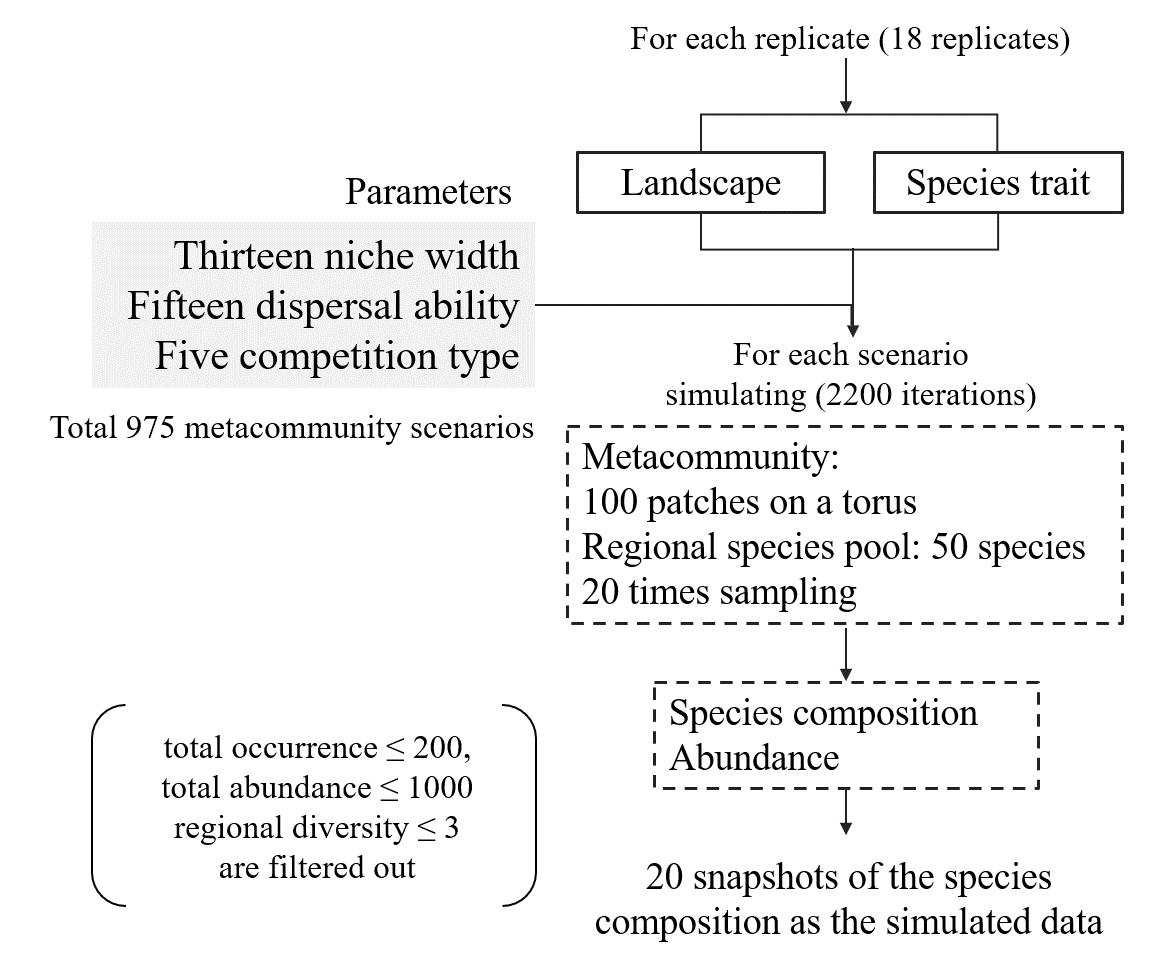
\includegraphics[width=0.7\linewidth]{./figures/ppt/Thompson.png}
	\caption[Flow diagram of process-based metacommunity framework in \citet{thompson2020process}.]{\small
		Flow diagram of process-based metacommunity framework in \citet{thompson2020process}. For each replicate, the coordinates and the environment of the patches, and the trait of species are independently generated before the iteration. The niche width, competition types and dispersal ability of the species are the parameters that regulated the ecological processes underlying the simulated metacommunity. After 2200 iterations, the simulation model generates maximally 100 nonempty patches on a torus. The regional species pool contains maximally 50 species. After the 1800th iteration, every 20 iterations we records the species composition and abundance of the species in each patch. Overall we get 20 snapshots of the species composition from a simulated metacommunity.}
	\label{fig:thompson}
\end{figure}


%%% d
\subsection{Simulation of metacommunity data with stochasticity}
\noindent
For each replicate of the simulation, the landscape configuration, including the coordinates of the patches and the environment value of each patch, and species trait are first generated before the iteration starts (Fig. \ref{fig:thompson}). The environment value in each patch is fixed across all the iterations. The initial species abundance of each species in each patch is generated independently by Poisson distribution with mean 0.5. The simulation ran 2200 iterations, with 200 iterations for the burn-in stage. Within the burn-in stage, the recruitment event, which adds individuals with numbers independently generated by Poisson distribution with mean 0.5 for each species in each patch, is implemented every 20 iterations. The number of individuals of species $i$ in patch $x$ in time $t$ ($t$-th iteration) is denoted by $N_{ix}(t)$. Then, the expected individual number of species $i$ in patch $x$ in time $t+1$ is defined as 
\[
N_{exp,ix}(t+1) = N_{ix}(t)\dfrac{r_{ix}(t)}{1+\sum_{j = 1}^S\alpha_{ij}N_{jx}(t)} - E_{ix}(t)+I_{ix}(t)
\]
The number of individuals of species $i$ in patch $x$ at time $t+1$ is generated by Poisson distribution with mean equal to the expected individual number at time $t$, i.e. $N_{ix}(t+1)\sim Poisson(N_{exp,ix}(t+1))$. After 1800 iterations, the abundance for each species in each patch was recorded until simulation ended for every 20 iterations. We eventually recorded 20 snapshots of the species composition and abundance of a simulated metacommunity ($t = 1,2,...,19,20$) (Fig. \ref{fig:thompson}). 

For each replicate, we simulated the metacommunity dynamics with the same parameters setting proposed by \citet{thompson2020process} (Fig. \ref{fig:thompson}). Thirteen values for niche width $\sigma$ were selected from 0.001 to 10. Fifteen values for dispersal ability $a$ were selected within 0.00001 to 1. The competition type was specified from one of the five scenarios mentioned in the \hyperref[Modelc]{previous section}. Eighteen replicates were run independently.

For further analysis, the samples with low species occurrence, diversity and abundance, i.e. total occurrence $\leq$ 200, total abundance $\leq$ 1000 or regional diversity $\leq$ 3, were excluded. Then, four metacommunity archetypes were defined subjectively by a specific combination of parameters in the parametric space. \textit{Patch dynamics} (PD) was defined as the one with competition-colonization trade-off and arbitrary determined niche width and dispersal ability; \textit{species sorting} (SS) were defined as the scenario in species with relatively narrow niche width, intermediate dispersal ability and stable competition; \textit{neutral dynamics} (ND) were defined as the one with relatively wide niche width, intermediate dispersal ability and no competition; \textit{mass effect} (ME) was defined as the one with relatively strong dispersal ability, narrow niche width and stable competition. These archetypes represented the extreme scenarios of the simulated metacommunity. They were the samples for testing the effect of the sampling effort and were also used for visualizing the dynamics of the summary statistics. The simulation in this section was run in \texttt{Julia} \citep{bezanson2017julia}.

%%%%% variation partitioning
\section{Beta-diversity variation partitioning}
\noindent
\label{sec:VP}
%%% a
%\subsection*{(a) Introduction: data inputs}
Beta-diversity variation partitioning is a popular method for quantifying the relative importance of environmental filtering and dispersal underlying species turnover. This method was proposed by \citet{borcard1992partialling} and has been widely used in ecological studies \citep{cottenie2005integrating, peres2006variation, smith2010variation}. The method is based on the constrained ordination technique, which quantifies the variation in species composition explained by environment and distance between plots. Species composition, environmental data and geographical information for each plot in the observed metacommunity are needed for this analytical method. The explained variation of environment and space may be further used to compare the relative importance of environmental filtering and dispersal in species turnover across metacommunities \citep{cottenie2005integrating}. However, several issues of variation partitioning have already been discussed \citep[chap.~4]{leibold2017metacommunity}. For example, the more complete the environmental data is, the higher may be the variation explained by the environment, which may even change the inference on which process is the most important \citep{chang2013better}. Another example is that the magnitude of the total variation of species composition may increase when the regional species pool is larger \citep{kraft2011disentangling}. In this case, with the fixed environmental and geographical variables, the unexplained variation of the species composition is expected to increase by chance \citep[pp.~124]{leibold2017metacommunity}.

%%% b
%\subsection*{(b) Analyzing procedure: CCA + dbMeM}
We calculated the summary statistics of beta-diversity variation partitioning for the simulated data generated in \autoref{sec:thom}. Canonical correspondence analysis (CCA) was considered in our study since we assumed that the response of the species to the environment in the simulation model is a Gaussian curve, not a linear line \citep{ter1986canonical, legendre2012numerical}. A snapshot of the species abundance matrix was assigned as the response variable, while environment values generated at the beginning of the simulation and spatial attributes derived from the coordinates of the patches were used as the explanatory variables in CCA. The spatial attributes were derived from applying distance-based Moran's eigenvector maps (dbMEM) on the distance matrix of the patches \citep{borcard2002all}. To quantify the pattern of positive autocorrelation in species abundances, only the eigenfunctions with positive eigenvalues were considered as the explanatory variables. The adjusted R-squared (adjusted R$^2$) \citep[pp.~633]{legendre2012numerical} derived from the variation partitioning in CCA represented: (1) variation explained only by the environment, fraction [a], (2) variation explained only by space, fraction [c], (3) variation explained by both environment and space, fraction [b], and (4) unexplained variation, fraction [d] (Fig. \ref{fig:VP}). We defined fractions [a], [b], [c] and [d] as the summary statistics of beta-diversity variation partitioning. These four partitions of variation were calculated by following: (1) fraction [a]+[b] is the adjusted R$^2$ with species composition as response variable and only environment as explanatory variable in CCA; (2) fraction [b]+[c] is the adjusted R$^2$ with species composition as response variable and only eigenfunctions corresponding to positive eigenvalues as explanatory variables in CCA; (3) fraction [a]+[b]+[c] is the adjusted R$^2$ with species composition as response variable and both environment and eigenfunctions corresponding to positive eigenvalues as explanatory variables in CCA; (4) fraction explained only by environment [a] is calculated by ([a]+[b]+[c])-([b]+[c]); (5) fraction explained only by space [c] is calculated by ([a]+[b]+[c])-([a]+[b]); (6) fraction explained by both environment and space [b] is calculated by ([a]+[b]+[c])-[a]-[c]; (7) unexplained fraction [d] is calculated by 1-([a]+[b]+[c]). All the calculation in this section was done in \texttt{R} \citep{R}.

\begin{figure}
	\centering
	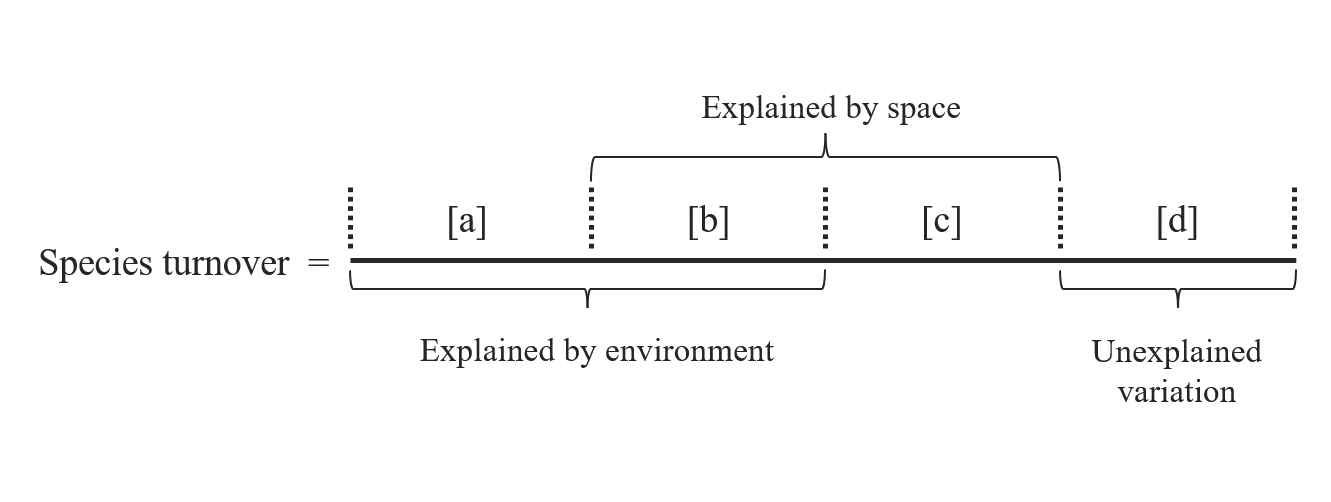
\includegraphics[width=\linewidth]{./figures/ppt/VP.png}
	\caption[Visualization of the statistics of beta-diversity variation partitioning.]{\small
		Visualization of the statistics of beta-diversity variation partitioning (modified Fig. 1 from \citealp{peres2006variation}). Fraction [a] represents the variation explained only by the environment, fraction [b] represents the variation explained only by space, fraction [c] represents the variation explained by both environment and space, and fraction [d] represents the unexplained variation. These four fractions are defined as the summary statistics of beta-diversity variation partitioning. See \autoref{sec:VP} for a detailed explanation.}
	\label{fig:VP}
\end{figure}

%%%%% Stegen
\section{Stegen's framework}
\noindent
\label{sec:Stegen}
%%% a
%\subsection*{(a) Introductions: data inputs}
\citet{stegen2013quantifying} is a null model-based method proposed to quantify the relative importance of selection, dispersal limitation, homogenizing dispersal and drift underlying the microbial metacommunity. Phylogenetic data and species composition data of the observed metacommunity are required in this framework. Compared to most of the null model-based methods that can only disentangle the presence of some ecological processes \citep{ulrich2010null, chase2011disentangling}, \citet{stegen2013quantifying} applied two-step null model to every pair of plots within the metacommunity. The significance of the divergence or the convergence of the phylogeny structure and species composition between the two plots was tested. The relative importance of the four ecological processes is summarized by the significances derived from all pairs (Fig. \ref{fig:stegen}). \citet{ford2020functional} modified Stegen's framework and used community-level functional trait data instead of phylogenetic data to quantify the relative importance of selection in the fish metacommunity. In our study, we used the trait-based modified version of Stegen's framework proposed by \citet{ford2020functional}.

\begin{figure}
	\centering
	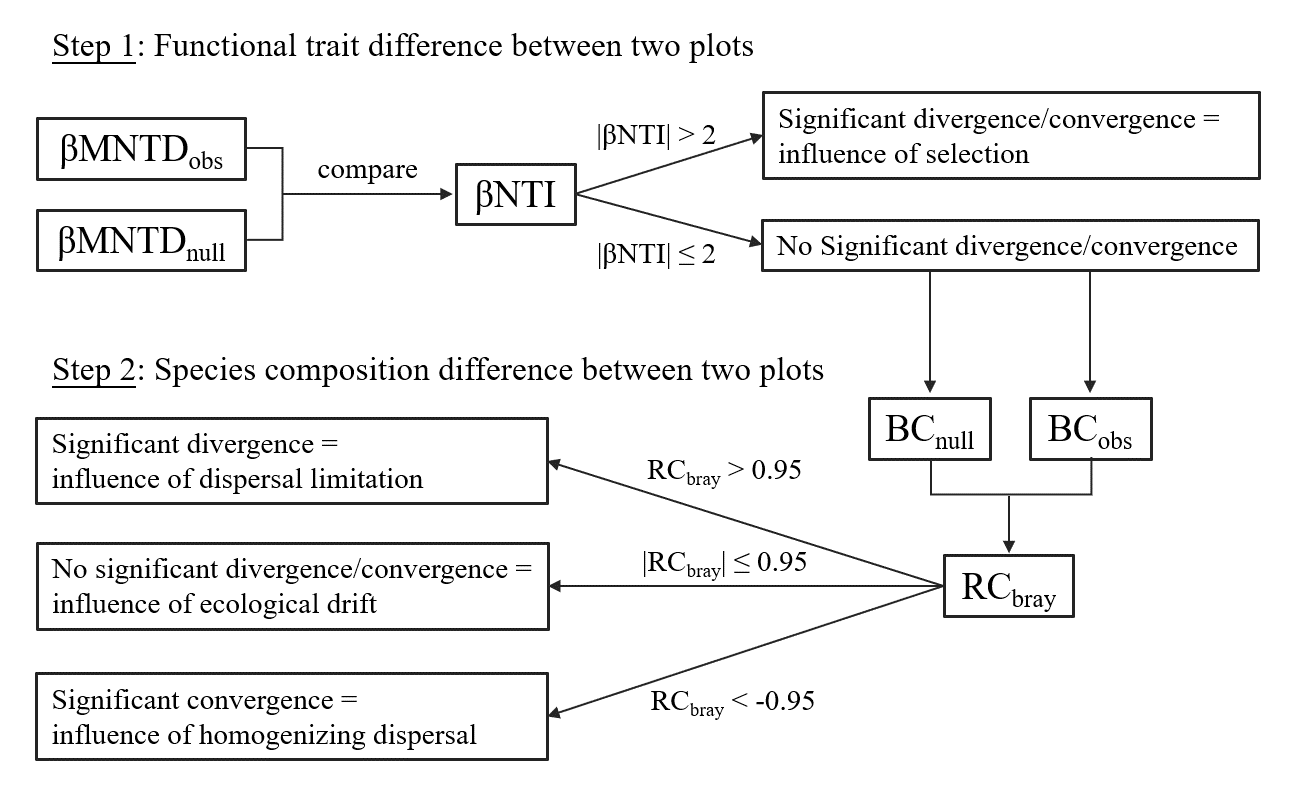
\includegraphics[width=\linewidth]{./figures/ppt/Stegen.png}
	\caption[Flow diagram of modified Stegen's framework of two-step null model.]{\small
		Flow diagram of modified Stegen's framework of two-step null model (modified Fig. 3 from \citet{stegen2013quantifying}). The relative importance of selection, dispersal limitation, ecological drift and homogenizing dispersal underlying the metacommunity are quantified based on the differences in functional traits and species composition between plots. These four values are defined as the summary statistics of modified Stegen's framework. See \autoref{sec:Stegen} for a detailed explanation.}
	\label{fig:stegen}
\end{figure}


%%% b
%\subsection*{(b) Details of procedures}
% first step
The framework proposed by \citet{stegen2013quantifying} and modified by \citet{ford2020functional} consists of two steps. In the first step, abundance-weighted $\beta$-mean-nearest taxon distance ($\beta$MNTD) quantifies the functional distance between two plots. $\beta$MNTD between plot $k$ and plot $m$ is 
\[
\beta \text{MNTD}_{km} = 0.5\cdot \left[\sum_{i_k = 1}^{n_k} f_{i_k}\min(\Delta_{i_k,m}) + \sum_{i_m = 1}^{n_m} f_{i_m}\min(\Delta_{i_m,k})\right]
\]
where $n_k$ is the number of species in plot $k$, $f_{i_k}$ is the relative abundance of $i_k$-th species in plot $k$ and $\min(\Delta_{i_k,m})$ is the minimum of trait difference between $i_k$-th species in plot $k$ and any species in plot $m$. To calculate the deviation of the observed $\beta$MNTD from the null model expectation, species traits are permuted, and $\beta$MNTD is recalculated by the permuted species traits. After repeating 999 times of permutation and recalculation, $\beta$-nearest taxon index ($\beta$NTI) is calculated by the difference of observed $\beta$MNTD and mean of the null model $\beta$MNTD in the unit of the standard deviation of $\beta$MNTD. If $\beta$NTI is larger than 2 or less than -2, then we conclude that the functional turnover is larger than expected and selection is the main process underlying this pair of plots. If $\beta$NTI is within -2 to 2, then go to the second step.

% second step
In the second step, the modified Raup-Crick probability metric (RC$_{bray}$) of \citet{chase2011disentangling} is applied to identify the most important process from the remaining processes, i.e. dispersal limitation, homogenizing dispersal, or drift. The Bray-Curtis distance between two plots is calculated first, and it is recalculated 999 times after the permutation in species abundance. The total abundance and number of species in each plot and the abundance of the species in the whole metacommunity are consistent in the permutation. The observed Bray-Curtis distance and the set of Bray-Curtis distances generated by the null model are combined and standardized into the range of -1 to 1. The modified Raup-Crick probability metric (RC$_{bray}$) is then the standardized observed Bray-Curtis distance. According to the thresholds introduced by \citet{chase2011disentangling}, if RC$_{bray}$ > 0.95, the main process underlying these two plots is dispersal limitation with drift. If RC$_{bray}$ < -0.95, homogenizing dispersal is the main process. If RC$_{bray}$ is within -0.95 and 0.95, pure drift is acting on the species turnover.

%%% outputs
%\subsection*{(c) Outputs: fractions as the statistics in the further analysis}
In our study, we applied this twe-step null model to all the possible pairs of patches in a simulated metacommunity, and calculated the relative importance (fraction) of selection, dispersal limitation with drift, homogenizing dispersal, and pure drift based on the species composition and species traits. These relative importances were treated as the summary statistics of Stegen's framework. All the calculation in this section was done in \texttt{Julia} \citep{bezanson2017julia}.

% DNCI
\section{Dispersal-niche continuum index (DNCI)}
\noindent
\label{sec:dnci}
% a
%\subsection*{(a) Introductions: inputs}
Dispersal-niche continuum index (DNCI) is another null model-based method that aims to quantify the relative importance of niche and dispersal assembly processes underlying the paleontological community data \citep{vilmi2021dispersal} (Fig. \ref{fig:DNCI}). Only grouped species composition data is required to calculate DNCI. This parsimony benefits understanding the ecological processes underlying the paleontological community, whose environment and functional trait data are difficult to collect. The group can be defined based on any cluster analysis or ordination methods.


%\subsection*{(b) Details of procedure}
To calculate DNCI for the simulated metacommunity, we clustered the patches within the metacommunity into two groups based on Ward's minimum variance method \citep[pp360]{legendre2012numerical}. Then the similarity percentage (SIMPER) of each species in the metacommunity, which indicates the contribution of the species to the overall average dissimilarity (OAD) between two groups of patches, was calculated \citep{clarke1993non}. The contribution of species $i$ to the dissimilarity between patch $j$ and $k$ is defined by \citet{clarke1993non} as the Bray-Curtis dissimilarity between patch $j$ and $k$:
\[
\delta_{jk(i)} = \dfrac{|y_{ij} - y_{ik}|}{\sum_{i=1}^p (y_{ij}+y_{ik})}
\]
where $y_{ij}$ and $y_{ik}$ are the abundance of species $i$ in patch $j$ and patch $k$ respectively; $p$ is the number of species in the metacommunity. The raw contribution of species $i$ to OAD $\overline{\delta_i}$ is defined as the average of the contribution of species $i$ to the dissimilarity between every pair of patches in different groups, i.e.
\[
\overline{\delta}_i = \dfrac{1}{M_1M_2}\sum_{\substack{j \in G_1\\ k \in G_2}}\delta_{jk(i)}
\]
where $G_1$ and $G_2$ are the set of patches in group 1 and group 2, and $M_1$ and $M_2$ are the numbers of patches in group 1 and group 2 respectively. The OAD $\overline{\delta}$ is defined by the summation of the raw contribution of all the species, i.e. $\overline{\delta} = \sum_{i=1}^p \overline{\delta}_i$. Finally, the SIMPER profile is derived from the decreasing ranking of the contribution ratio of the species $\overline{\gamma}_i = \overline{\delta}_i/\overline{\delta}$.

Three null models are implemented to disentangle the effect of niche and dispersal assembly processes. Let's suppose that the species composition is with rows as patches and columns as species. The first null hypothesis is $H_{0d}$: only dispersal assembly processes are driving the species turnover within the metacommunity. Under this null hypothesis, the column sum is constrained, and within each column, the abundances are permuted among all patches independently. Additionally, the sum of the abundances of all the species within each plot is constrained to be nonzero. In this case, the total abundance of each species in the metacommunity is kept constant but there may be a different number of individuals and species in a single patch in every permutation. The second null hypothesis was $H_{0n}$: only niche assembly processes are driving the species turnover within the metacommunity. Under this null hypothesis, the row sum was constrained, and within each row, the abundances were permuted independently. In this case, the sum of the abundances of all species in each patch was kept constant, but the total abundance of any of the species is likely to vary in every permutation. The third null hypothesis is $H_{0dn}$: both dispersal and niche assembly processes are driving the species turnover in the metacommunity. Under this null hypothesis, the species composition matrix was permuted with constrained column sum and row sum. Under each of these three null hypotheses, the species composition matrix was permuted 99 times and the SIMPER profile was recalculated by using the permuted species composition. The permutation with three different types of constraint is implemented by the function \texttt{permatfull()} in package \texttt{vegan} in \texttt{R} \citep{R}. To compare the observed SIMPER profile with each null SIMPER profile, the logarithm of the sum of squared deviations $E$ was calculated: 
\[
E = \log_{10}(\sum_{i=1}^p(\overline{\gamma}_{i,null} - \overline{\gamma}_{i,obs})^2)
\]
Finally, for each null hypothesis, we got 99 $E$ values, which were denoted by $E_{d(q)}$, $E_{n(q)}$ and $E_{dn(q)}$, for $H_{0d}$, $H_{0n}$ and $H_{0dn}$, and $q$ is the index from 1 to 99. The standard effect sizes ($SES$) of $E_d$ and $E_n$ are defined as the mean of the standardized $E_d$ and $E_n$:
\[
SES_d = \frac{1}{Q}\sum_{q=1}^Q \dfrac{E_{d(q)} - \overline{E}_{dn}}{\sigma_{dn}} = \frac{1}{Q}\sum_{q=1}^Q SES_{d(q)}
\]
\[
SES_n = \frac{1}{Q}\sum_{q=1}^Q \dfrac{E_{n(q)} - \overline{E}_{dn}}{\sigma_{dn}} = \frac{1}{Q}\sum_{q=1}^Q SES_{n(q)}
\]
where $Q$ is the total number of permutations plus one, which is 100, $\overline{E}_{dn}$ is the mean of $E_{dn(q)}$ and $\sigma_{dn}$ is the standard deviation of $E_{dn(q)}$. In the end, the dispersal-niche continuum index (DNCI) is defined as
\[
\text{DNCI} = SES_d - SES_n
\]
and its standard deviation is defined as the squared root of the sum of the square of the standard deviation of the standardized $E_d(q)$ and $E_n(q)$:
\[
\sigma_{\text{DNCI}} = \sqrt{\sigma^2(SES_{d(q)}) + \sigma^2(SES_{n(q)})}
\]
The width of the confidence interval of DNCI is defined as $2\sigma_{\text{DNCI}}$.


% outputs
%\subsection*{(c) Outputs}
DNCI and its standard deviation were used to infer the relative importance of dispersal and niche assembly processes underlying the metacommunity. If DNCI is significantly larger than 0, then niche assembly processes are the dominant processes driving the species turnover. If DNCI is significantly lower than 0, then dispersal assembly processes are the most influential in affecting species composition. If DNCI is not significantly different from 0, then both these two processes may be similarly important for the community assembly. The significance is determined by whether the confidence interval of DNCI encompasses 0. In our study, we treated DNCI and its standard deviation as the summary statistics of the metacommunity. Additionally, since in some cases, the species composition was too sparse (contained too many zeros) and failed to find the column permutation with nonzero row sums, we added the time limitation that if the permutation cannot be found in 30 seconds then we dropped that whole sample. All the calculation in this section was done in \texttt{R} \citep{R}.


\begin{figure}
	\centering
	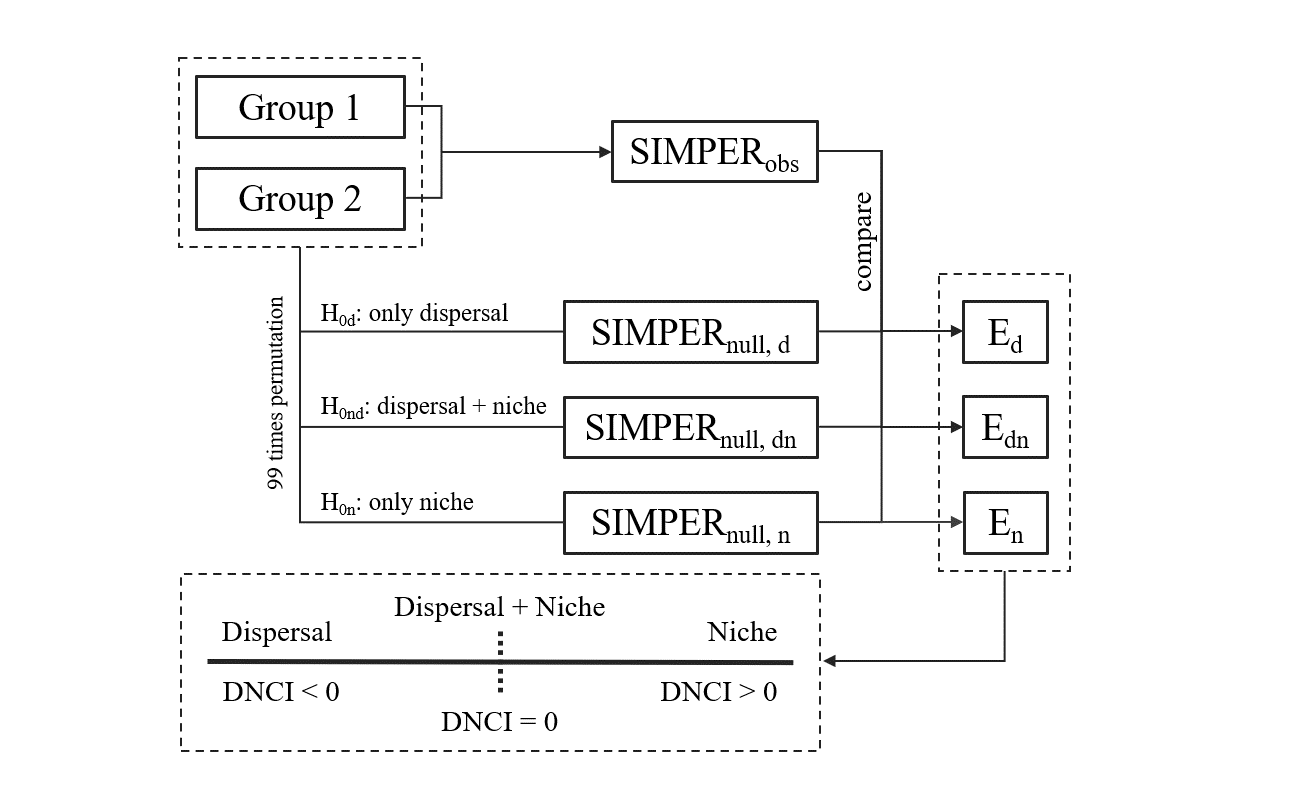
\includegraphics[width=\linewidth]{./figures/ppt/DNCI.png}
	\caption[Flow diagram for calculating dispersal-niche continuum index.]{\small
		Flow diagram for calculating dispersal-niche continuum index (modified Fig. 1 from \citet{vilmi2021dispersal}). By studying the contribution of the species to the dissimilarity within the metacommunity, the relative importance of dispersal and niche assembly processes can be identified by the dispersal-niche continuum index (DNCI). Positive DNCI represents the metacommunity is mainly driven by niche assembly processes; negative DNCI represents the metacommunity is mainly driven by dispersal assembly processes. DNCI and its standard deviation are defined as the summary statistics of these analytical methods. See \autoref{sec:dnci} for a detailed explanation.}
	\label{fig:DNCI}
\end{figure}

%%%%% Random forest
\section{Random forest approach linking summary statistics with parametric space}
\noindent
%%% intro
%\subsection*{(a) Introduction}
Random forest (RF) is a statistical classifier that constructs a mapping between variables by the training data. The correctness of classification and prediction can be quantified by giving the testing data. We applied this statistical approach to construct the link between the summary statistics, which are derived from beta-diversity variation partitioning, Stegen's framework and DNCI, and the model parameters in \citeauthor{thompson2020process}'s process-based metacommunity framework. The trained RF were then applied to the empirical data to disentangle underlying the ecological processes.


%\subsection*{(b) Procedure}
To construct the RF, the first 12 replicates of the simulated data (two-thirds of 18 replicates) were used as the training data and the last 6 replicates of them were used as the testing data. The response variables were the model parameters that influenced the relative importance of ecological processes underlying the metacommunity: niche width, competition type and dispersal ability of the species. Niche width and dispersal ability were treated as ordinal variables \citep{hornung2020ordinal}, and competition type was treated as a categorical variable. We constructed 12 RFs for each model parameter. The explanatory variables of these RFs consisted of four sets of summary statistics and three sets of time steps. We considered the summary statistics derived from only beta-diversity variation partitioning, only Stegen's framework, only DNCI or all three analytical methods with one snapshot ($t = 20$), four snapshots ($t = 20, 16, 12, 8$) or all 20 snapshots of the species composition as the explanatory variables. To evaluate the prediction of the trained RFs, the statistics calculated by the testing data were then entered into the trained RFs, and the accuracy of prediction was estimated by the proportion of the correct link between the prediction of the parameter and the exact model parametric setting. The importance of each explanatory variable, i.e. the statistics derived from the analytical methods, in predicting the model parameters was quantified. For predicting competition type, the importance of the explanatory variables was defined by the mean decrease Gini \citep{han2016variable}, which was derived from the component \texttt{importance} of the object \texttt{randomForest} in \texttt{R}. For predicting niche width and dispersal ability, the importance of the explanatory variables was defined by the permutation variable importance measure \citep{janitza2016random}, which was derived from the component \texttt{varimp} of the object \texttt{ordfor} in \texttt{R}.

Without interpolating, a complete data (with no missing values) is required for constructing and evaluating the RF. Only the samples without missing summary statistics at all 20 periods were used to construct and evaluate the RFs. The missing statistics in some samples at some periods may be caused by the strong stochasticity, which produced the low occurrences, diversity and abundance metacommunities, and the sparseness of the species composition, which resulted in the lack of DNCI.

% sensitivity
\section{Sensitivity analysis to sampling effort and choice of time steps}
\noindent
The robustness of the RFs with summary statistics derived from all three analytical methods at four snapshots to the sampling effort was evaluated. Four archetypes, \textit{species sorting} (SS), \textit{neutral dynamics} (ND), \textit{mass effect} (ME) and \textit{patch dynamics} (PD), were determined by a point in the parametric space defined by dispersal ability, niche width and competition type after the simulation (see \autoref{sec:thom} for details). For the sake of reducing the calculation time, we only considered these four archetypes in the last six replicates as the testing data. We calculated the summary statistics for the four snapshots ($t = 20, 16, 12, 8$) of the simulated species composition generated by the parameters setting of these four archetypes based on the three analytical methods. Then we subsampled the species composition data by randomly choosing 10, 20, ..., and 90 of the patches 15 times independently. For different sampling efforts, the summary statistics were recalculated based on the subsampled species composition and inserted in the trained RF to calculate the accuracy in predicting the model parameters.

We evaluated the robustness of the same RF to the choice of the time steps to be the training data. The explanatory variables of the RF were the summary statistics derived by the three analytical methods from the snapshots at $t = 20, 16, 12, 8$. For each model parameter (niche width, dispersal ability and competition type), we treated the summary statistics at randomly chosen four time steps from $t = 1, 2,\dots, 19, 20$ as the inputs of the trained RF. The correctness of the prediction based on the mismatched summary statistics was calculated. We randomly chose the time steps 1000 times. The distribution of the accuracy for predicting three model parameters was shown in the boxplot.

\section{Application on Fushan Forest Dynamics Plot}
\noindent
The Fushan Forest Dynamics Plot (FDP) is a 25-ha forest dynamics plot established in northern Taiwan in 2004. FDP is located in the subtropical zone at 24˚45'40"N, 121˚33'28"E with elevation from 600 to 733 m.a.s.l. The 500 m x 500 m plot is devided into 625 20 m x 20 m quadrates. The delineation of the plot was conducted in 2002-2003. Precise topography was measured by the electronic total-station theodolites. FDP consists of multiple topographic components, such as hills, ridges, slopes, valleys, flats and creeks. Mean elevation, convexity, slope and aspect of each quadrat were considered as the environmental data of FDP \citep{su2007fushan}. 

The species composition of FDP was surveyed in 2003-2004, 2008-2009, 2013-2014 and 2018-2019, following the method developed by the Center for Tropical Forest Science (CTFS, now ForestGEO) \citep{condit1998tropical}. These four censuses were imagined as the four snapshots of the Fushan forest. All the woody species and the tree ferns with a diameter at breast height (DBH) of $\geq$ 1 cm were identified, measured, mapped and tagged. Within four censuses of FDP, between 111,000 to 134,000 individuals of 111 species in 40 families and 68 genera were recorded. Three species of tree ferns, \textit{Cyathea lepifera}, \textit{C. podophylla} and \textit{C. spinulosa} were removed from the further analysis since they are not woody species. The individuals which were missing (status = -1) or lost their stem without DBH of its branches $\geq$ 1 cm (status = -2) were removed from the quadrat in the species composition. Details of the information about environmental conditions and the field survey can be found in \citet{su2007fushan}.

Leaf traits were measured on the randomly selected 6-12 individuals for each species found in the FDP. Specific leaf area (SLA), leaf thickness and leaf dry matter content (LDMC) for 103 specie were obtained based on the established protocols for measuring leaf functional traits \citep{hrguindeguy2013new}. Total organic nitrogen mass per unit leaf mass (N mass) and total organic phosphorus mass per unit leaf mass (P mass) were obtained for 99 of the 103 species based on two microplate methods. The maximum tree height of the 99 species was measured according to the established protocols. The wood density of 74 species was measured in Fushan, of 21 species were obtained from the literature in Taiwan. The wood density of the remaining species was derived from \citet{chave2009towards}.

The species composition, topographical data and coordinates of each quadrat and traits data for each species were used to calculate the summary statistics of beta-diversity variation partitioning, Stegen's framework and DNCI. Since the incompleteness in trait data, when calculating the dissimilarity of traits between two plots in Stegen's framework ($\beta$MNTD), the species with missing traits were ignored. We obtained four sets of summary statistics based on the four snapshots of the species composition in FDP. These summary statistics were inputted into the trained random forest incorporating the three analytical methods and four snapshots with tested performance and robustness to the sampling effort and choice of time steps. Then, the competition types, niche width and dispersal ability of the species in the Fushan forest were estimated.

\setcounter{section}{0}  
% !TeX root = ../main.tex
\chapter*{3. Results}
\setcounter{chapter}{3}
\addcontentsline{toc}{chapter}{3. Results}
\section{Summary of the simulated data}
\noindent
Overall, we had 17,500 samples from 18 replicates of metacommunity with 975 scenarios (5 competition types, 15 dispersal ability types and 13 niche widths) generated by \citeauthor{thompson2020process}'s framework. Each sample contained 20 snapshots of the species composition at different time steps. After filtering out the incomplete samples, which missed some summary statistics, we retained 5983 samples and 399 scenarios and used them in further analysis.

The parametric space for the retained samples was shown by heat map (Fig. \ref{fig:para}). The scenarios with weak dispersal ability $a$ and narrow niche width $\lambda$ were mostly filtered out. Parametric space defined by dispersal ability $a$ and niche width $\lambda$ was wider in scenarios of no competition, stable competition and equal competition (Fig. \ref{fig:para-no}, \ref{fig:para-stable}, \ref{fig:para-equal}), compared to mixed competition and competition-colonization trade-off (Fig. \ref{fig:para-mixed}, \ref{fig:para-CC}). We defined four metacommunity archetypes based on the parametric space (Fig. \ref{fig:para-arch}).

%
\begin{figure}
	\centering
	\begin{subfigure}[b]{0.45\linewidth}
		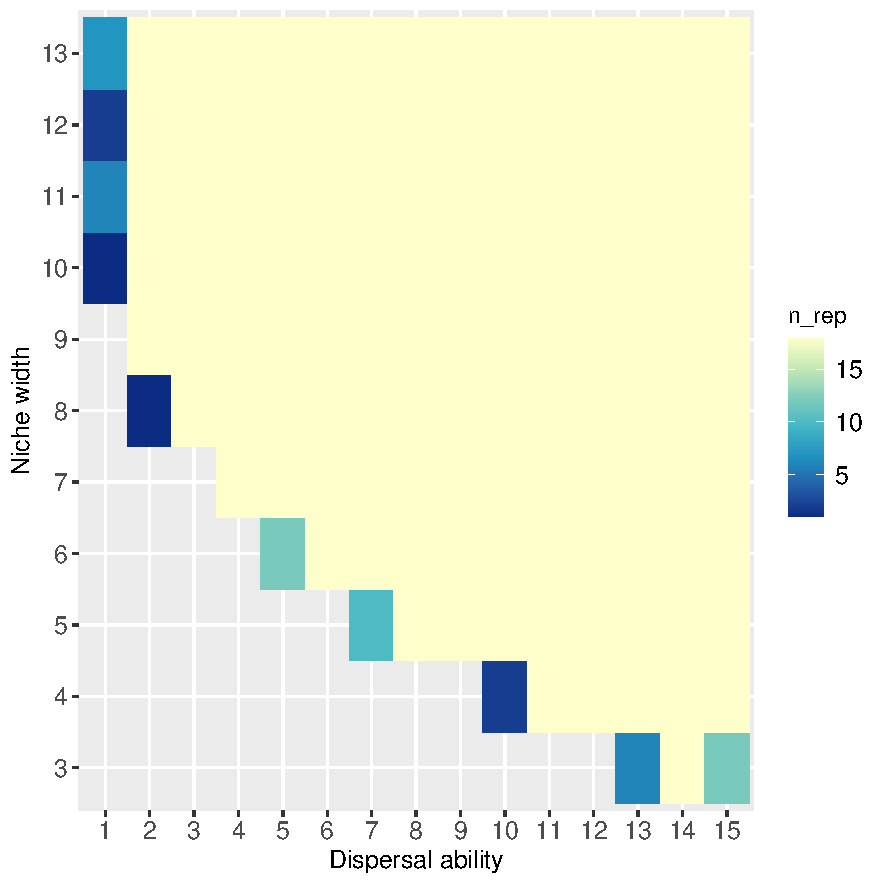
\includegraphics[width=\linewidth]{./figures/Parameter_space_overlook_no_competition.pdf}
		\caption{No competition}
		\label{fig:para-no}
	\end{subfigure}
	\begin{subfigure}[b]{0.45\linewidth}
		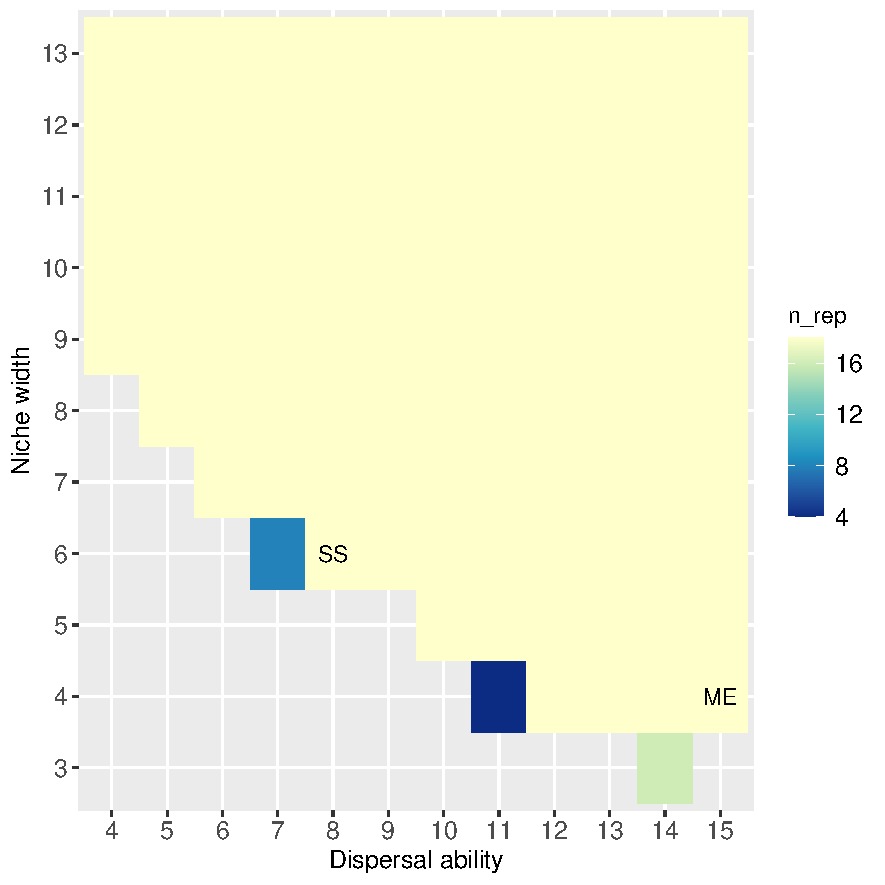
\includegraphics[width=\linewidth]{./figures/Parameter_space_overlook_stable_competition.pdf}
		\caption{Stable competition}
		\label{fig:para-stable}
	\end{subfigure}
	\begin{subfigure}[b]{0.45\linewidth}
		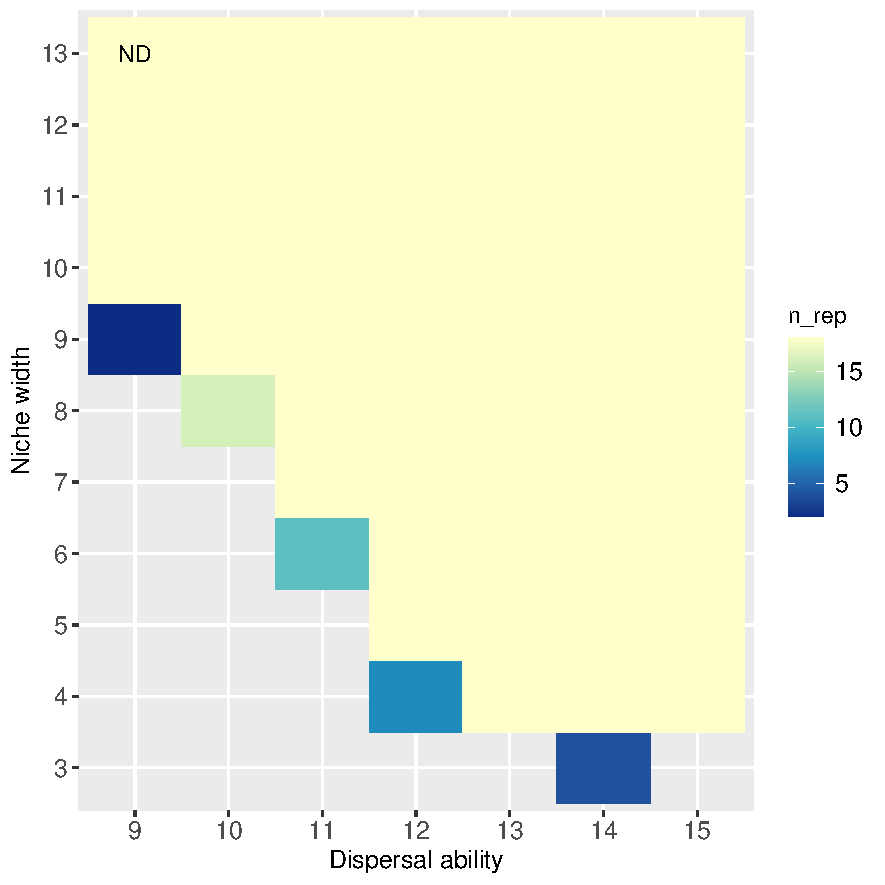
\includegraphics[width=\linewidth]{./figures/Parameter_space_overlook_equal_competition.pdf}
		\caption{Equal competition}
		\label{fig:para-equal}
	\end{subfigure}
	\begin{subfigure}[b]{0.45\linewidth}
		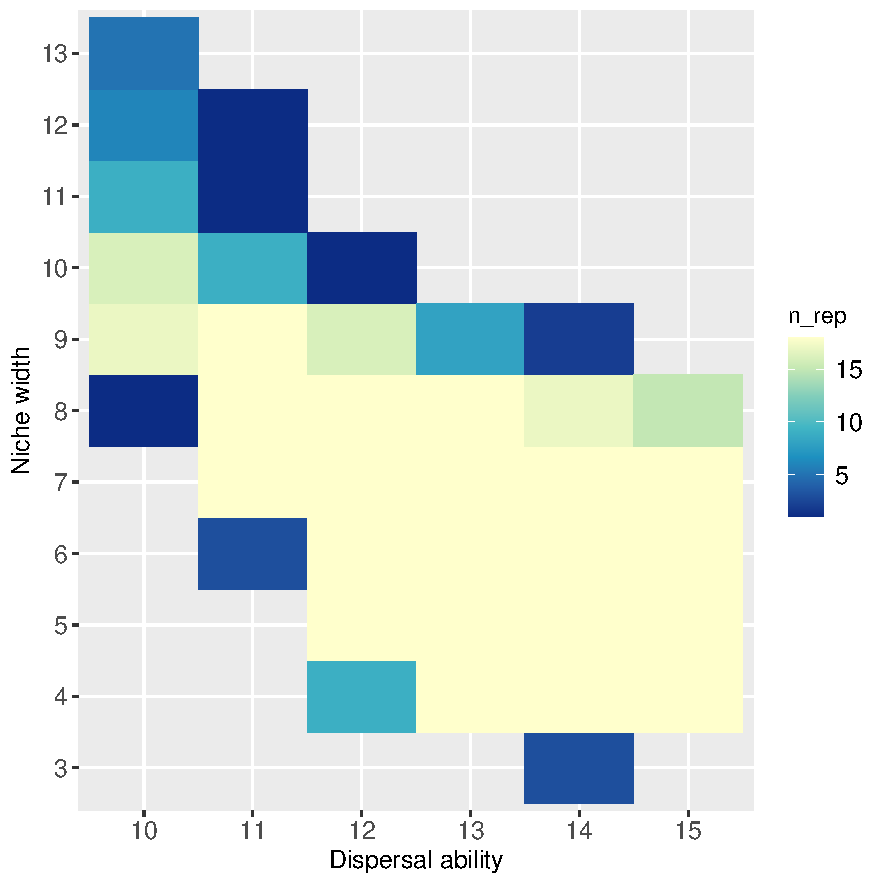
\includegraphics[width=\linewidth]{./figures/Parameter_space_overlook_mixed_competition.pdf}
		\caption{mixed competition}
		\label{fig:para-mixed}
	\end{subfigure}
\end{figure}
\begin{figure}\ContinuedFloat
	\centering
	\begin{subfigure}[b]{0.45\linewidth}
		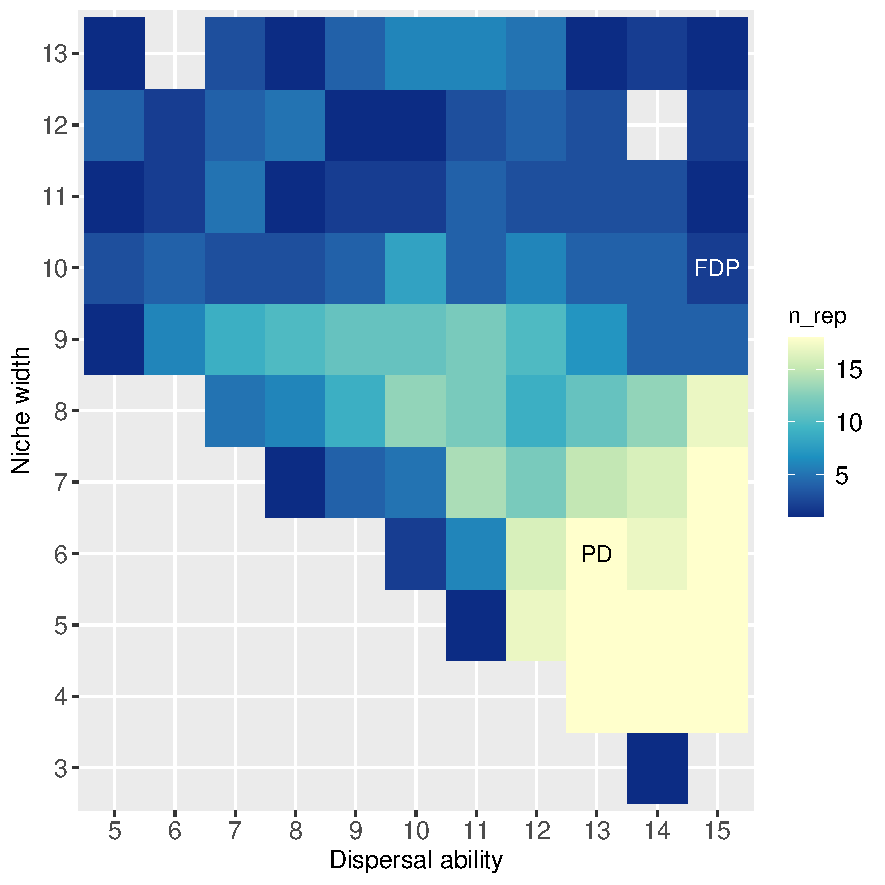
\includegraphics[width=\linewidth]{./figures/Parameter_space_overlook_CC_tradeoff.pdf}
		\caption{CC trade-off}
		\label{fig:para-CC}
	\end{subfigure}
	\begin{subfigure}[b]{0.45\linewidth}
		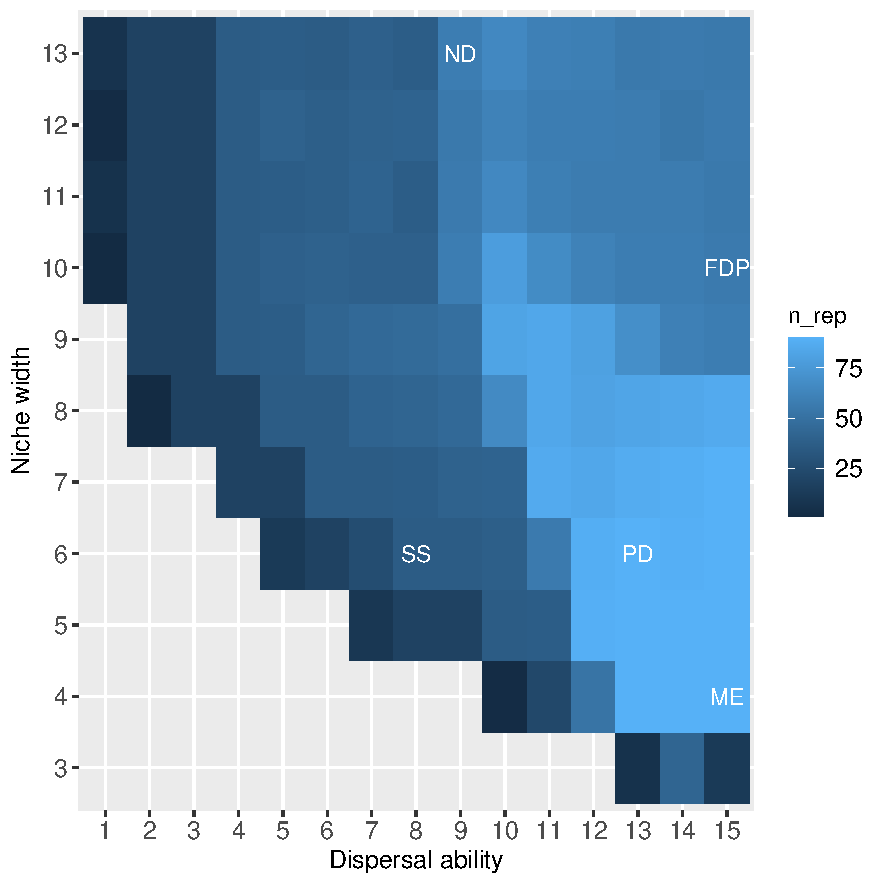
\includegraphics[width=\linewidth]{./figures/Parameter_space_overlook_archetypes.pdf}
		\caption{Archetypes}
		\label{fig:para-arch}
	\end{subfigure}
	\caption[Parametric space defined by niche width, dispersal ability and competition type.]{\small
		Parametric space defined by niche width, dispersal ability and competition type. The number on the two axes represents the level of the niche width and dispersal ability. On the x-axis, the numbers from 1 to 15 are the dispersal ability from weak to strong. On the y-axis, the numbers from 1 to 13 are the niche widths from narrow to wide. The values in the tile plots represent the number of replicates that remain after excluding those with too low species abundance, diversity and occurrence, or those too sparse to calculate DNCI. If the scenario has no replicates after filtering, the values are shown as missing in the tile plots. The axes are truncated since no replicates remained after data filtering for those scenarios. Panels (a)-(e) show the parameter space defined by niche width and dispersal ability with different competition types. Panel (f) is the summation of the five tile plots from (a) to (e). The labels in the tile plot show the subjective definition of the four metacommunity archetypes in the parametric space: \textit{species sorting} (SS), \textit{neutral dynamics} (ND), \textit{mass effect} (ME) and \textit{patch dynamics} (PD). The species in the Fushan Forest Dynamics Plot (FDP) are predicted to interact with each other with competition-colonization trade-off, average strong dispersal ability and wide niches.}
	\label{fig:para}
\end{figure}
%

\section{Summary statistics of the simulated metacommunity}
\noindent
Statistics of beta-diversity variation partitioning, DNCI and Stegen's framework were calculated for the remaining 5983 samples. All the statistics fluctuated across time and differed between replicates (Fig. \ref{fig:stat_comp}). The summary statistics derived from Stegen's frame could successfully separate the four archetypes. The relative importance of selection could separate SS and ND from each other; the relative importance of homogenizing dispersal could separate ME and ND; the relative importance of drift could separate PD and SS. In beta-diversity variation partitioning, only ND could be separated from the other archetypes based on unexplained variation. DNCI could not identify any archetypes.

The ranges of the summary statistics of three analytical methods were calculated (Tab. \ref{tbl:sum_stat}). The reason that the minimal value of the variation explained only by environment, only by space, and by both environment and space derived from the variation partitioning was negative was that the explained variation was calculated by the adjusted R$^2$ which may be negative when R$^2$ is extremely close to zero \citep[pp.~633]{legendre2012numerical}. The maximum value of residual derived from variation partitioning could be larger than 1 because the residual was calculated by 1 minus the sum of the explained variation by either environment or space. The statistics derived from Stegen's framework ranged from 0 to 1. DNCI and its standard deviation had no boundary limitation. The average and standard deviation were also calculated for each summary statistic.

% figure: comparing different archetypes
\begin{figure}
	\centering
	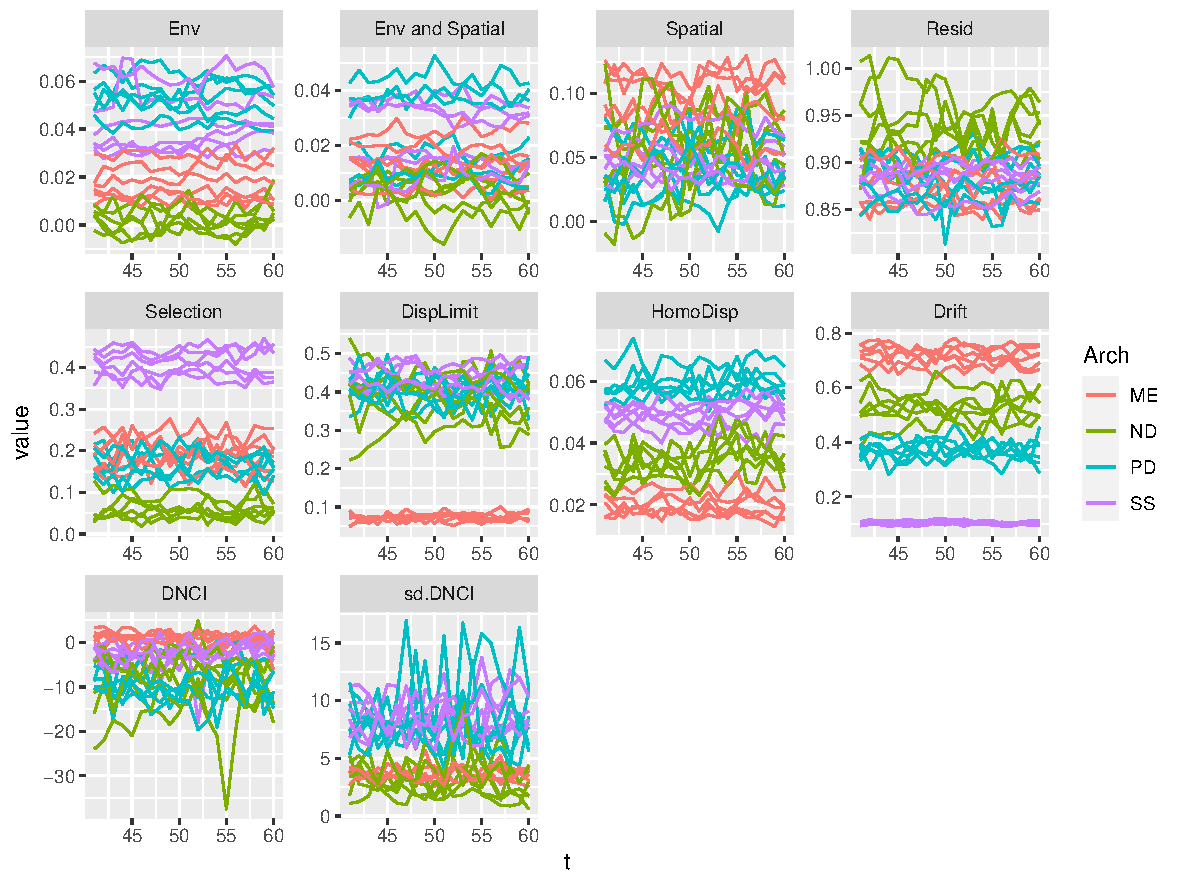
\includegraphics[width=\textwidth]{./figures/Compare_archetypes_six_rep.pdf}
	\caption[Comparing the dynamics of the summary statistics derived by beta-diversity variation partitioning, Stegen's framework and DNCI under four metacommunity archetypes.]{\small
		Comparing the dynamics of the summary statistics derived by beta-diversity variation partitioning, Stegen's framework and DNCI under four metacommunity archetypes. Within each panel, the curve shows the dynamics of the values of each summary statistic across time. The first row shows the dynamics of the variation explained only by the environment [a], by both environment and space [b], only by space [c], and unexplained variation [d] derived from beta diversity variation partitioning. The second row shows the dynamics of the fraction of selection, dispersal limitation, homogenizing dispersal, and drift derived from Stegen's framework. The third row shows the dynamics of DNCI and its standard deviation. Different colors represent different metacommunity archetypes. A maximum of six replicates are shown for each archetype.}
	\label{fig:stat_comp}
\end{figure}

% table: Overview of the summary statistics
\afterpage{
	\begin{footnotesize}
		% table: performance
		\setlength\tabcolsep{1.5pt}
		\begin{longtable}{l|rrrrrrrrrr}
			\caption[Overview of all statistics derived by beta-diversity variation partitioning, Stegen's framework and DNCI]{\small
				Overview of all statistics derived by beta-diversity variation partitioning, Stegen's framework and DNCI. For the description of the statistics please see the caption of Fig. \ref{fig:stat_comp}.}
			\label{tbl:sum_stat}
			\endfirsthead
			\toprule
			\multicolumn{1}{l}{} & \multicolumn{4}{c}{Stegen} & \multicolumn{4}{c}{VP} &  &  \\ 
			\cmidrule(lr){2-5} \cmidrule(lr){6-9}
			\multicolumn{1}{l}{} & Selection & DispLimit & HomoDisp & Drift & Env & Env and Spatial & Spatial & Resid & DNCI & sd.DNCI \\ 
			\midrule
			Min & 0.00 & 0.00 & 0.00 & 0.04 & -0.01 & -0.09 & -0.16 & 0.14 & -383.48 & 0.02 \\ 
			Max & 0.78 & 0.94 & 0.66 & 0.99 & 0.64 & 0.51 & 0.43 & 1.16 & 298.89 & 146.72 \\ 
			Mean & 0.15 & 0.27 & 0.05 & 0.53 & 0.07 & 0.05 & 0.06 & 0.82 & -7.60 & 2.31 \\ 
			Sd & 0.18 & 0.22 & 0.05 & 0.28 & 0.09 & 0.07 & 0.05 & 0.18 & 15.00 & 3.43 \\ 
			\bottomrule
		\end{longtable}
	\end{footnotesize}
}
%


\section{Performance in prediction model parameters}
\noindent
The accuracy in predicting the process parameters was quantified for all 12 random forests (RFs) (Tab. \ref{tbl:rf}). Among 12 RFs, the one that embedded all statistics of 20 snapshots had the highest accuracy in predicting dispersal ability (71.92\%) and niche width (72.02\%). This RF also had the second-highest accuracy in predicting competition type (87.49\%), which was only 0.31\% less than the RF with the highest accuracy. The second best RF was the one with all summary statistics at four snapshots as the explanatory variables, which had 68.61\%, 71.97\% and 87.80\% correction rates in predicting the dispersal ability, niche width and competition type, respectively. For the RFs that only considered one analytical method, Stegen's framework had the highest accuracy in predicting all three model parameters compared to beta-diversity variation partitioning and DNCI with the same number of snapshots. However, the RFs which integrated statistics derived from multiple analytical methods had better accuracy than those which only considered statistics derived from single analytical methods in predicting the model parameters.

The importance of the explanatory variables of the RF that incorporates the summary statistics derived from three different analytical methods based on the four snapshots was quantified (Tab. \ref{tbl:impo}). The fraction of homogenizing dispersal and selection derived from Stegen's framework and the standard deviation of DNCI were the most three important statistics for predicting the competition type. The fraction of selection, homogenizing dispersal and dispersal limitation derived from Stegen's framework and the variation explained by space derived from variation partitioning were the most important statistics for predicting dispersal ability. Variation explained only by environment, the fraction of selection and drift derived from Stegen's framework were the most important statistics for predicting niche width.

%
%

\section{Robustness to the sampling effort and choice of time steps}
\noindent
For the trained RF with summary statistics derived by three analytical methods from four snapshots, the accuracy for predicting the niche width, dispersal ability and competition type decreased when the sampling effort decreased (Fig. \ref{fig:robust-samp}). However, the accuracy for predicting the dispersal ability, niche width and competition type had no difference even though the summary statistics were derived from the species composition at four randomly selected time steps (Fig. \ref{fig:robust-time}). 

\begin{figure}
	\centering
	\begin{subfigure}[b]{0.47\textwidth}
		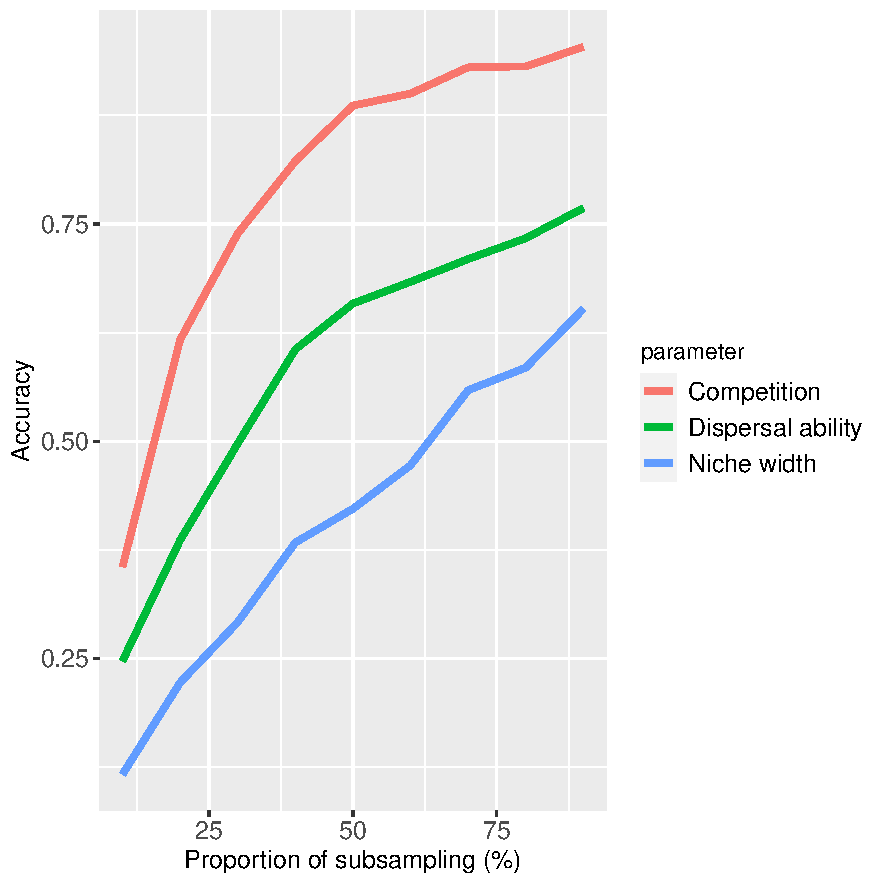
\includegraphics[width=\textwidth]{./figures/Robustness_sampling_effort_Accuracy.pdf}
		\caption{Sampling effort}
		\label{fig:robust-samp}
	\end{subfigure}
	\begin{subfigure}[b]{0.47\textwidth}
		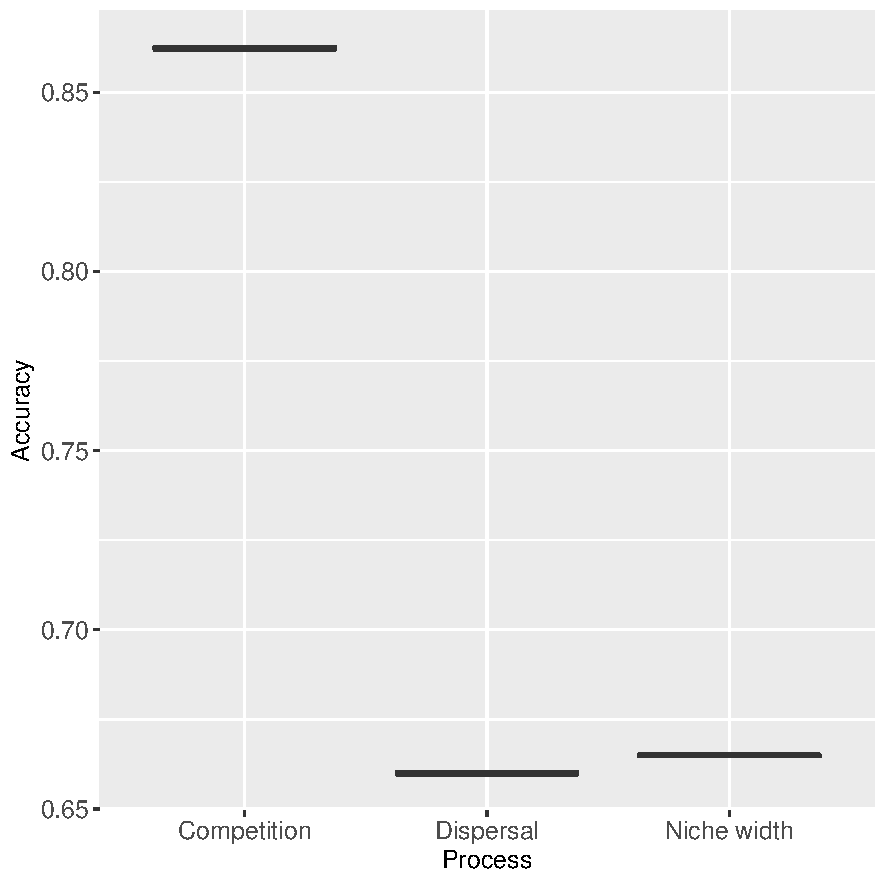
\includegraphics[width=\textwidth]{./figures/Robustness_time_step_Accuracy_distribution.pdf}
		\caption{Choice of time steps}
		\label{fig:robust-time}
	\end{subfigure}
	\caption[Robustness of random forest to the sampling effort and choice of the time steps.]{\small
		Robustness of random forest (RF) to the sampling effort and choice of the time steps. (a) Different curves represent the relationship between the accuracy for predicting competition type, niche width and dispersal ability, and proportion of the subsampled patches from a whole simulated metacommunity. (b) The distribution of the accuracy of the RF for predicting competition type, niche width and dispersal ability when using the summary statistics at the randomly chosen time steps. The variance of the accuracy is considerably small that is not visible in the boxplots displayed.}
	\label{fig:robust}
\end{figure}
%

% table: performance
\afterpage{%
	\begin{small}
		\begin{longtable}{lrrrrrrrrrr}
			\caption[Accuracy of 12 RFs with different explanatory variables in prediction model parameters.]{\small
				Accuracy of 12 RFs with different explanatory variables in prediction model parameters. The first four columns show the explanatory variables in the RFs. The symbol "O" represents the summary statistics derived from which analytical methods are considered in the RF. The symbol "X" represented they are not considered in the RF. The fourth column represented how many snapshots of the species composition are used to calculate the summary statistics and considered as the explanatory variables in the RF. The accuracy for predicting dispersal ability, niche width and competition type is shown in the last 3 columns. VP: beta-diversity variation partitioning. Stegen: Stegen's framework. DNCI: DNCI and its standard deviation.}
			\label{tbl:rf}
			\endfirsthead
			\toprule
			\multicolumn{4}{c}{Explanatory variables} &  &  &  \\ 
			\cmidrule(lr){1-4}
			\multicolumn{3}{c}{Summary statistics} &  & \multicolumn{3}{c}{Performance of prediction} \\ 
			\cmidrule(lr){1-3} \cmidrule(lr){5-7}
			VP & Stegen & DNCI & Snapshots & Dispersal ability & Niche width & Competition type \\ 
			\midrule
			O & X & X & 1 & 18.83\% & 42.59\% & 45.86\% \\ 
			O & X & X & 4 & 21.95\% & 50.83\% & 56.40\% \\ 
			O & X & X & 20 & 24.01\% & 52.13\% & 60.32\% \\ 
			X & O & X & 1 & 45.10\% & 46.91\% & 69.46\% \\ 
			X & O & X & 4 & 53.14\% & 53.74\% & 77.00\% \\ 
			X & O & X & 20 & 57.36\% & 53.24\% & 78.96\% \\ 
			X & X & O & 1 & 18.08\% & 23.96\% & 45.76\% \\ 
			X & X & O & 4 & 26.27\% & 29.43\% & 55.80\% \\ 
			X & X & O & 20 & 30.79\% & 32.95\% & 59.87\% \\ 
			O & O & O & 1 & 61.07\% & 69.61\% & 84.43\% \\ 
			O & O & O & 4 & 68.61\% & 71.97\% & 87.80\% \\ 
			O & O & O & 20 & 71.92\% & 72.02\% & 87.49\% \\ 
			\bottomrule
		\end{longtable}
	\end{small}
}


\section{Application to Fushan Forest Dynamics Plot}
\noindent
By inputting the summary statistics derived from four snapshots of the FDP by three analytical methods (Tab. \ref{tbl:empirical}), we estimated that the species in the FDP act with competition-colonization trade-off and strong average dispersal ability and wide niche width (Fig. \ref{fig:para-CC}). 

%

\newpage
\chapter*{4. Discussions}
\setcounter{chapter}{4}
\addcontentsline{toc}{chapter}{4. Discussions}
\noindent
Multiple analytical methods were introduced to derive summary statistics from the observational data to quantify the ecological information of the observed metacommunity and disentangle the underlying ecological processes. However, a single analytical method on a snapshot of the metacommunity has unsatisfying performance in predicting the underlying processes was shown in \citet{guzman2022accounting} and confirmed in our study. Within the three analytical methods considered in our study, we showed that only Stegen's framework could successfully separate the four metacommunity archetypes, which were arbitrarily defined to represent the extreme scenarios of the simulated metacommunity (Fig. \ref{fig:stat_comp}). Even though Stegen's framework could successfully separate the four archetypes, its performance in predicting the precise underlying processes was still unsatisfying. By integrating more analytical methods applied on multiple snapshots of the metacommunity, the prediction of the underlying processes may be improved. 

RF was used to link the summary statistics derived from the analytical methods with the model parameters in a process-based simulation model. We showed that this technique successfully integrates multiple analytical methods to disentangle the ecological processes underlying the observed metacommunity in \citeauthor{guzman2022accounting}'s framework. From the application of this framework in the observational data, we showed that competition-colonization trade-off was identified among the species in the Fushan Forest Dynamics Plot (FDP). This trade-off suggests competition hierarchy and a trade-off between the ability of competition and colonization among the species. The competition hierarchy between species may indicate that the FDP is composed of early-successional and late-successional species. Late-successional species may be missing in some areas of this forest plot because of the frequent impact of typhoons during summer, which creates empty patches for the early-successional species to establish. The frequent impacts of typhoons may be also the reason for the strong stochasticity and weak deterministic effect of the environmental conditions we found in the FDP, which are indicated by the predicted wide niches of the species. Strong average dispersal ability may result in the high occurrence of the common species, e.g. \textit{Blastus cochinchinensis} (柏拉木) and \textit{Helicia formosana} (山龍眼). 

This practical demonstration is missing in \citet{guzman2022accounting}. In our study, we showed that \citeauthor{guzman2022accounting}'s framework may be applied to disentangle the ecological processes underlying the observed metacommunity by plotting it onto the parametric space. However, several issues need to be considered.

First, the assumptions of the process-based simulation model should align with the observed metacommunity. In our study, \citeauthor{thompson2020process}'s metacommunity simulation model considers species as annual plants that die in each iteration, which may not correctly represent the long-living woody plant species in the FDP. The impact of this mismatch on the results is unknown and requires further investigation. Additionally, we assumed constant environmental conditions in our simulated metacommunity over time. This assumption may not be satisfied for the marine and tidal ecosystems whose environmental conditions in the local communities are intensively fluctuating. Furthermore, we assumed all the species had the same niche width and dispersal ability. To release this assumption for modeling a more complex system, we may assume that the niche width and the dispersal ability of the species are followed normal distributions with adjustable mean and variance. Since the model assumptions and the parametric space are determined before the simulation and construction of the RFs, any changes are expected to influence the parameter estimation and its accuracy. Hence, the accuracy of the RF in predicting the model parameters may not be compared across process-based simulation models with different model assumptions and parametric spaces.

Second, the process-based simulation model should generate a relatively complete range of summary statistics. Any statistics which can be derived from both simulated data and observed data could be the explanatory variables in the RF. However, if the statistics calculated by the observed data are not encompassed within the extent that the simulation model can generate, the prediction may be unreasonable. In our study, the determined parametric space in the simulation model generated a relatively complete range of summary statistics derived from the three analytical methods. Moreover, the summary statistics calculated by the observational data from the FDP were encompassed within the range of summary statistics. In \citet{guzman2022accounting}, the descriptive statistics were included as the explanatory variables of the RF. However, some of the descriptive statistics are intensively varied across systems and may not be easily controlled in the process-based simulation model. For example, gamma diversity is one of the descriptive statistics of the metacommunity. It may not only be regulated by the strength of ecological processes, but also by the size of the species pool and the number of patches of the simulated metacommunity. Without modifying these two parameters in our study, the range of the gamma diversity derived from the simulated data would be limited and may not encompass the gamma diversity derived from the observed metacommunity. 

Third, the incompleteness of the observed data may influence the accuracy of parameter estimation. We showed that the incompleteness of the species composition reduced the performance of the trained RF in predicting the model parameters. In practice, because of the variety of functional responses and resource types, we can never measure all types of traits and environmental variables. This incompleteness of the community data may cause deviation in summary statistics. For example, the unmeasured environmental variables are shown to considerably influence the summary statistics of the beta-diversity variation partitioning \citep{chang2013better}. We expect this deviation may lead to the performance of the trained RF being overestimated. The magnitude of the deviation is determined by the robustness of the analytical methods themselves. Thus, the robustness of the analytical methods should be compared systematically, and the summary statistics that are too sensitive to the incompleteness of the data should be excluded from the set of explanatory variables.

Fourth, the choice of the time steps to calculate the summary statistics as the explanatory variables of the RF may influence the parameter estimation. The simulation models are likely to generate more snapshots of the species composition than is usually available for observed data. The training data of the RF is determined by the summary statistics calculated by the simulated data at the arbitrarily chosen time steps. Moreover, the number of the chosen time steps should be identical to the census times of the observed metacommunity. However, in practice, we usually do not know which time steps in the simulation model represent which census of the observed metacommunity. We showed that even though the time steps to calculate the statistics as the inputs of the RF were randomly chosen, the performance of the RF was maintained. If the summary statistics have no stable trends across time, we expect that the choice of the time steps may influence the parameter estimation, and such statistics should be excluded from the explanatory variables of the RF.

\chapter*{5. Future Directions}
\setcounter{chapter}{5}
\addcontentsline{toc}{chapter}{5. Future Directions}
\noindent
We demonstrated \citeauthor{guzman2022accounting}'s framework in disentangling the ecological processes underlying the observed metacommunity. In practice, the process-based simulation model can be modified or replaced based on different focuses on the ecological processes and different types of ecosystems. \citeauthor{thompson2020process}'s model is principally based on high-level ecological processes and is sufficiently general to be applied to different community systems. By modeling more detailed ecological processes, e.g. how seed germination and variation in the mortality rate in seedling and juvenile stage would influence the colonization of the species or releasing the assumption of identical niche width and dispersal ability of the species, we may understand more about under what processes allow different species assemble to become a community and metacommunity. However, the trade-off between generality, realism, and precision cannot be ignored \citep{levins1966strategy}. Constructing a comprehensive and complex process-based model may result in losing its generality to apply to different ecosystems and reduce the precision in estimating the model parameters. In this case, we should generate more training data or apply a more powerful technique for parameter estimation. Besides, the sets of analytical methods for predicting the strength of ecological processes may be considered based on the availability of the data. For instance, if the functional traits data of the species are not available, the trait-based analytical methods, i.e. modified Stegen's framework, cannot be applied. 

Except for RF, there are also other approaches to estimate the parameters in a process-based stochastic model \citep{hartig2011statistical}. For example, approximation Bayesian computation (ABC) is a rejection algorithm for estimating the parameters in the process-based simulation model based on summary statistics \citep{csillery2010approximate}. \citet{van2015new} applied ABC to quantify the strength of limiting similarity, dispersal assembly and filtering underlying the observed metacommunities based on the functional diversity metrics. \citet{ruffley2019identifying} compared and incorporated RF and ABC to quantify the strength of competition and environmental filtering based on the information about phylogeny, functional traits and phylogenetic signals within the traits of the local community. Different statistical classifiers may be compared and incorporated to improve the performance in estimating the model parameters. Alternatively, cross-validation may be further applied to find the subset of the explanatory variables that maximize the performance.

Improving the framework for better disentangling the underlying ecological processes is essential for understanding and predicting how anthropogenic activity and climate change affect the species composition, diversity and ecosystem services. By estimating the model parameters based on the metacommunities across changes in environmental conditions, we may study how the strength of the ecological processes is altered by anthropogenic activity and climate change. We may further predict the dynamics of the metacommunity based on the process-based model with estimated model parameters to reach better principles for conservation.




\chapter*{Conclusions}
\setcounter{chapter}{6}
\addcontentsline{toc}{chapter}{Conclusions}
\noindent
\citet{guzman2022accounting} provided a framework that may integrate multiple analytical methods and multiple snapshots of the observational metacommunity to disentangle the ecological processes underlying the observed metacommunity. Our study demonstrates this framework in practice by the observational data from the Fushan forest and shows the competition-colonization trade-off among species and the strong stochasticity and dispersal ability of the species in the Fushan forest. The performance of this framework in quantifying the strength of the ecological processes may be evaluated. However, this performance may be overestimated because of the incompleteness of the observational data and the inference of this framework may be influenced by the assumptions of the process-based simulation model.


\section*{Data availability}
\noindent
All the codes may be found in: \url{https://github.com/ChingLinHuang/Code-for-Master-Thesis}.


% 參考文獻
% References
\refmatter
%\bibliographystyle{ecollet}
%\bibliography{citation} % check .bbl file and copy to ref.tex
\begin{thebibliography}{70}
	\expandafter\ifx\csname natexlab\endcsname\relax\def\natexlab#1{#1}\fi
	
	\bibitem[{Adler \emph{et~al.}(2010)Adler, Ellner \&
		Levine}]{adler2010coexistence}
	Adler, P.B., Ellner, S.P. \& Levine, J.M. (2010).
	\newblock Coexistence of perennial plants: an embarrassment of niches.
	\newblock \emph{Ecology Letters}, 13, 1019--1029.
	
	\bibitem[{Adler \emph{et~al.}(2007)Adler, HilleRisLambers \&
		Levine}]{adler2007niche}
	Adler, P.B., HilleRisLambers, J. \& Levine, J.M. (2007).
	\newblock A niche for neutrality.
	\newblock \emph{Ecology Letters}, 10, 95--104.
	
	\bibitem[{Bezanson \emph{et~al.}(2017)Bezanson, Edelman, Karpinski \&
		Shah}]{bezanson2017julia}
	Bezanson, J., Edelman, A., Karpinski, S. \& Shah, V.B. (2017).
	\newblock Julia: A fresh approach to numerical computing.
	\newblock \emph{SIAM Review}, 59, 65--98.
	
	\bibitem[{Borcard \& Legendre(2002)}]{borcard2002all}
	Borcard, D. \& Legendre, P. (2002).
	\newblock All-scale spatial analysis of ecological data by means of principal
	coordinates of neighbour matrices.
	\newblock \emph{Ecological Modelling}, 153, 51--68.
	
	\bibitem[{Borcard \emph{et~al.}(1992)Borcard, Legendre \&
		Drapeau}]{borcard1992partialling}
	Borcard, D., Legendre, P. \& Drapeau, P. (1992).
	\newblock Partialling out the spatial component of ecological variation.
	\newblock \emph{Ecology}, 73, 1045--1055.

	\bibitem[{Borics \emph{et~al.}(2020)Borics, B-B{\'e}res, B{\'a}csi, Luk{\'a}cs,
  	T-Krasznai, Botta-Duk{\'a}t \& V{\'a}rb{\'\i}r{\'o}}]{borics2020trait}
	Borics, G., B-B{\'e}res, V., B{\'a}csi, I., Luk{\'a}cs, B.A., T-Krasznai, E.,
  	Botta-Duk{\'a}t, Z. \& V{\'a}rb{\'\i}r{\'o}, G. (2020).
	\newblock Trait convergence and trait divergence in lake phytoplankton reflect
  	community assembly rules.
	\newblock \emph{Scientific Reports}, 10, 19599.
	
	\bibitem[{ter Braak(1986)}]{ter1986canonical}
	ter Braak, C.J. (1986).
	\newblock Canonical correspondence analysis: a new eigenvector technique for
	multivariate direct gradient analysis.
	\newblock \emph{Ecology}, 67, 1167--1179.
	
	\bibitem[{Brown \emph{et~al.}(2017)Brown, Sokol, Skelton \&
		Tornwall}]{brown2017making}
	Brown, B.L., Sokol, E.R., Skelton, J. \& Tornwall, B. (2017).
	\newblock Making sense of metacommunities: dispelling the mythology of a
	metacommunity typology.
	\newblock \emph{Oecologia}, 183, 643--652.
	
	\bibitem[{Chang \emph{et~al.}(2013)Chang, Zelený, Li, Chiu \&
		Hsieh}]{chang2013better}
	Chang, L.-W., Zelený, D., Li, C.-F., Chiu, S.-T. \& Hsieh, C.-F. (2013).
	\newblock Better environmental data may reverse conclusions about niche-and
	dispersal-based processes in community assembly.
	\newblock \emph{Ecology}, 94, 2145--2151.
	
	\bibitem[{Chase \emph{et~al.}(2020)Chase, Jeliazkov, Ladouceur \&
		Viana}]{chase2020biodiversity}
	Chase, J.M., Jeliazkov, A., Ladouceur, E. \& Viana, D.S. (2020).
	\newblock Biodiversity conservation through the lens of metacommunity ecology.
	\newblock \emph{Annals of the New York Academy of Sciences}, 1469, 86--104.
	
	\bibitem[{Chase \& Myers(2011)}]{chase2011disentangling}
	Chase, J.M. \& Myers, J.A. (2011).
	\newblock Disentangling the importance of ecological niches from stochastic
	processes across scales.
	\newblock \emph{Philosophical Transactions of the Royal Society B: Biological
		Sciences}, 366, 2351--2363.
	
	\bibitem[{Chave \emph{et~al.}(2009)Chave, Coomes, Jansen, Lewis, Swenson \&
		Zanne}]{chave2009towards}
	Chave, J., Coomes, D., Jansen, S., Lewis, S.L., Swenson, N.G. \& Zanne, A.E.
	(2009).
	\newblock Towards a worldwide wood economics spectrum.
	\newblock \emph{Ecology Letters}, 12, 351--366.
	
	\bibitem[{Chave \emph{et~al.}(2002)Chave, Muller-Landau \&
		Levin}]{chave2002comparing}
	Chave, J., Muller-Landau, H.C. \& Levin, S.A. (2002).
	\newblock Comparing classical community models: theoretical consequences for
	patterns of diversity.
	\newblock \emph{The American Naturalist}, 159, 1--23.
	
	\bibitem[{Chesson(2000)}]{chesson2000mechanisms}
	Chesson, P. (2000).
	\newblock Mechanisms of maintenance of species diversity.
	\newblock \emph{Annual Review of Ecology and Systematics}, pp. 343--366.
	
	\bibitem[{Clark \emph{et~al.}(2001)Clark, Carpenter, Barber, Collins, Dobson,
		Foley, Lodge, Pascual, Pielke~Jr, Pizer \emph{et~al.}}]{clark2001ecological}
	Clark, J.S., Carpenter, S.R., Barber, M., Collins, S., Dobson, A., Foley, J.A.,
	Lodge, D.M., Pascual, M., Pielke~Jr, R., Pizer, W. \emph{et~al.} (2001).
	\newblock Ecological forecasts: an emerging imperative.
	\newblock \emph{Science}, 293, 657--660.
	
	\bibitem[{Clarke(1993)}]{clarke1993non}
	Clarke, K.R. (1993).
	\newblock Non-parametric multivariate analyses of changes in community
	structure.
	\newblock \emph{Australian Journal of Ecology}, 18, 117--143.
	
	\bibitem[{Condit(1998)}]{condit1998tropical}
	Condit, R. (1998).
	\newblock \emph{Tropical forest census plots: methods and results from Barro
		Colorado Island, Panama and a comparison with other plots}.
	\newblock Springer Science \& Business Media.
	
	\bibitem[{Connolly \emph{et~al.}(2017)Connolly, Keith, Colwell \&
		Rahbek}]{connolly2017process}
	Connolly, S.R., Keith, S.A., Colwell, R.K. \& Rahbek, C. (2017).
	\newblock Process, mechanism, and modeling in macroecology.
	\newblock \emph{Trends in Ecology \& Evolution}, 32, 835--844.
	
	\bibitem[{Connor \& Simberloff(1979)}]{connor1979assembly}
	Connor, E.F. \& Simberloff, D. (1979).
	\newblock The assembly of species communities: chance or competition?
	\newblock \emph{Ecology}, 60, 1132--1140.
	
	\bibitem[{Cottenie(2005)}]{cottenie2005integrating}
	Cottenie, K. (2005).
	\newblock Integrating environmental and spatial processes in ecological
	community dynamics.
	\newblock \emph{Ecology Letters}, 8, 1175--1182.
	
	\bibitem[{Csill{\'e}ry \emph{et~al.}(2010)Csill{\'e}ry, Blum, Gaggiotti \&
		Fran{\c{c}}ois}]{csillery2010approximate}
	Csill{\'e}ry, K., Blum, M.G., Gaggiotti, O.E. \& Fran{\c{c}}ois, O. (2010).
	\newblock Approximate bayesian computation (abc) in practice.
	\newblock \emph{Trends in Ecology \& Evolution}, 25, 410--418.
	
	\bibitem[{Diamond(1975)}]{diamond1975island}
	Diamond, J.M. (1975).
	\newblock The island dilemma: lessons of modern biogeographic studies for the
	design of natural reserves.
	\newblock \emph{Biological Conservation}, 7, 129--146.
	
	\bibitem[{Evans(2012)}]{evans2012modelling}
	Evans, M.R. (2012).
	\newblock Modelling ecological systems in a changing world.
	\newblock \emph{Philosophical Transactions of the Royal Society B: Biological
		Sciences}, 367, 181--190.
	
	\bibitem[{Ford \& Roberts(2020)}]{ford2020functional}
	Ford, B.M. \& Roberts, J.D. (2020).
	\newblock Functional traits reveal the presence and nature of multiple
	processes in the assembly of marine fish communities.
	\newblock \emph{Oecologia}, 192, 143--154.
	
	\bibitem[{Fukami(2015)}]{fukami2015historical}
	Fukami, T. (2015).
	\newblock Historical contingency in community assembly: integrating niches,
	species pools, and priority effects.
	\newblock \emph{Annual Review of Ecology, Evolution, and Systematics}, 46,
	1--23.
	
	\bibitem[{Gibert \& Escarguel(2019)}]{gibert2019per}
	Gibert, C. \& Escarguel, G. (2019).
	\newblock PER-SIMPER—a new tool for inferring community assembly processes
	from taxon occurrences.
	\newblock \emph{Global Ecology and Biogeography}, 28, 374--385.
	
	\bibitem[{Gotelli \& McGill(2006)}]{gotelli2006null}
	Gotelli, N.J. \& McGill, B.J. (2006).
	\newblock Null versus neutral models: what's the difference?
	\newblock \emph{Ecography}, 29, 793--800.
	
	\bibitem[{Gotelli \& Ulrich(2012)}]{gotelli2012statistical}
	Gotelli, N.J. \& Ulrich, W. (2012).
	\newblock Statistical challenges in null model analysis.
	\newblock \emph{Oikos}, 121, 171--180.
	
	\bibitem[{Gravel \emph{et~al.}(2006)Gravel, Canham, Beaudet \&
		Messier}]{gravel2006reconciling}
	Gravel, D., Canham, C.D., Beaudet, M. \& Messier, C. (2006).
	\newblock Reconciling niche and neutrality: the continuum hypothesis.
	\newblock \emph{Ecology Letters}, 9, 399--409.
	
	\bibitem[{Guzman \emph{et~al.}(2022)Guzman, Thompson, Viana, Vanschoenwinkel,
		Horv{\'a}th, Ptacnik, Jeliazkov, Gasc{\'o}n, Lemmens, Anton-Pardo
		\emph{et~al.}}]{guzman2022accounting}
	Guzman, L.M., Thompson, P.L., Viana, D.S., Vanschoenwinkel, B., Horv{\'a}th,
	Z., Ptacnik, R., Jeliazkov, A., Gasc{\'o}n, S., Lemmens, P., Anton-Pardo, M.
	\emph{et~al.} (2022).
	\newblock Accounting for temporal change in multiple biodiversity patterns
	improves the inference of metacommunity processes.
	\newblock \emph{Ecology}, 103.
	
	\bibitem[{Han \emph{et~al.}(2016)Han, Guo \& Yu}]{han2016variable}
	Han, H., Guo, X. \& Yu, H. (2016).
	\newblock Variable selection using mean decrease accuracy and mean decrease
	gini based on random forest.
	\newblock In: \emph{2016 7th IEEE International Conference on Software
		Engineering and Service Science (ICSESS)}. IEEE, pp. 219--224.
	
	\bibitem[{Hartig \emph{et~al.}(2011)Hartig, Calabrese, Reineking, Wiegand \&
		Huth}]{hartig2011statistical}
	Hartig, F., Calabrese, J.M., Reineking, B., Wiegand, T. \& Huth, A. (2011).
	\newblock Statistical inference for stochastic simulation models--theory and
	application.
	\newblock \emph{Ecology Letters}, 14, 816--827.
	
	\bibitem[{Hodgson \& Halpern(2019)}]{hodgson2019investigating}
	Hodgson, E.E. \& Halpern, B.S. (2019).
	\newblock Investigating cumulative effects across ecological scales.
	\newblock \emph{Conservation Biology}, 33, 22--32.
	
	\bibitem[{Hornung(2020)}]{hornung2020ordinal}
	Hornung, R. (2020).
	\newblock Ordinal forests.
	\newblock \emph{Journal of Classification}, 37, 4--17.
	
	\bibitem[{Hubbell(2011)}]{hubbell2011unified}
	Hubbell, S.P. (2011).
	\newblock \emph{The Unified Neutral Theory of Biodiversity and Biogeography}.
	\newblock Princeton University Press.
	
	\bibitem[{Janitza \emph{et~al.}(2016)Janitza, Tutz \&
		Boulesteix}]{janitza2016random}
	Janitza, S., Tutz, G. \& Boulesteix, A.L. (2016).
	\newblock Random forest for ordinal responses: prediction and variable
	selection.
	\newblock \emph{Computational Statistics \& Data Analysis}, 96, 57--73.
	
	\bibitem[{Ke \emph{et~al.}(2015)Ke, Miki \& Ding}]{ke2015soil}
	Ke, P.-J., Miki, T. \& Ding, T.-S. (2015).
	\newblock The soil microbial community predicts the importance of plant traits
	in plant--soil feedback.
	\newblock \emph{New Phytologist}, 206, 329--341.
	
	\bibitem[{Kraft \emph{et~al.}(2015)Kraft, Adler, Godoy, James, Fuller \&
		Levine}]{kraft2015community}
	Kraft, N.J., Adler, P.B., Godoy, O., James, E.C., Fuller, S. \& Levine, J.M.
	(2015).
	\newblock Community assembly, coexistence and the environmental filtering
	metaphor.
	\newblock \emph{Functional Ecology}, 29, 592--599.
	
	\bibitem[{Kraft \emph{et~al.}(2011)Kraft, Comita, Chase, Sanders, Swenson,
		Crist, Stegen, Vellend, Boyle, Anderson
		\emph{et~al.}}]{kraft2011disentangling}
	Kraft, N.J., Comita, L.S., Chase, J.M., Sanders, N.J., Swenson, N.G., Crist,
	T.O., Stegen, J.C., Vellend, M., Boyle, B., Anderson, M.J. \emph{et~al.}
	(2011).
	\newblock Disentangling the drivers of $\beta$ diversity along latitudinal and
	elevational gradients.
	\newblock \emph{Science}, 333, 1755--1758.
	
	\bibitem[{Legendre \& Legendre(2012)}]{legendre2012numerical}
	Legendre, P. \& Legendre, L. (2012).
	\newblock \emph{Numerical ecology}.
	\newblock Elsevier.
	
	\bibitem[{Leibold \& Chase(2017)}]{leibold2017metacommunity}
	Leibold, M.A. \& Chase, J.M. (2017).
	\newblock \emph{Metacommunity Ecology}.
	\newblock Princeton University Press.
	
	\bibitem[{Leibold \emph{et~al.}(2004)Leibold, Holyoak, Mouquet, Amarasekare,
		Chase, Hoopes, Holt, Shurin, Law, Tilman
		\emph{et~al.}}]{leibold2004metacommunity}
	Leibold, M.A., Holyoak, M., Mouquet, N., Amarasekare, P., Chase, J.M., Hoopes,
	M.F., Holt, R.D., Shurin, J.B., Law, R., Tilman, D. \emph{et~al.} (2004).
	\newblock The metacommunity concept: a framework for multi-scale community
	ecology.
	\newblock \emph{Ecology Letters}, 7, 601--613.
	
	\bibitem[{Levins(1966)}]{levins1966strategy}
	Levins, R. (1966).
	\newblock The strategy of model building in population biology.
	\newblock \emph{American Scientist}, 54, 421--431.
	
	\bibitem[{MacArthur \& Levins(1967)}]{macarthur1967limiting}
	MacArthur, R. \& Levins, R. (1967).
	\newblock The limiting similarity, convergence, and divergence of coexisting
	species.
	\newblock \emph{The American Naturalist}, 101, 377--385.
	
	\bibitem[{MacArthur(1958)}]{macarthur1958population}
	MacArthur, R.H. (1958).
	\newblock Population ecology of some warblers of northeastern coniferous
	forests.
	\newblock \emph{Ecology}, 39, 599--619.
	
	\bibitem[{MacArthur \& Wilson(1967)}]{macarthur1967theory}
	MacArthur, R.H. \& Wilson, E.O. (1967).
	\newblock \emph{The Theory of Island Biogeography}.
	\newblock Princeton University Press.
	
	\bibitem[{Mayfield \& Levine(2010)}]{mayfield2010opposing}
	Mayfield, M.M. \& Levine, J.M. (2010).
	\newblock Opposing effects of competitive exclusion on the phylogenetic
	structure of communities.
	\newblock \emph{Ecology Letters}, 13, 1085--1093.
	
	\bibitem[{McGill(2010)}]{mcgill2010towards}
	McGill, B.J. (2010).
	\newblock Towards a unification of unified theories of biodiversity.
	\newblock \emph{Ecology Letters}, 13, 627--642.
	
	\bibitem[{McGill \emph{et~al.}(2006)McGill, Maurer \&
		Weiser}]{mcgill2006empirical}
	McGill, B.J., Maurer, B.A. \& Weiser, M.D. (2006).
	\newblock Empirical evaluation of neutral theory.
	\newblock \emph{Ecology}, 87, 1411--1423.
	
	\bibitem[{Molina \& Stone(2020)}]{molina2020difficulties}
	Molina, C. \& Stone, L. (2020).
	\newblock Difficulties in benchmarking ecological null models: an assessment of
	current methods.
	\newblock \emph{Ecology}, 101, e02945.
	
	\bibitem[{Ning \emph{et~al.}(2019)Ning, Deng, Tiedje \& Zhou}]{ning2019general}
	Ning, D., Deng, Y., Tiedje, J.M. \& Zhou, J. (2019).
	\newblock A general framework for quantitatively assessing ecological
	stochasticity.
	\newblock \emph{Proceedings of the National Academy of Sciences}, 116,
	16892--16898.
	
	\bibitem[{Ovaskainen \emph{et~al.}(2017)Ovaskainen, Tikhonov, Norberg,
		Guillaume~Blanchet, Duan, Dunson, Roslin \& Abrego}]{ovaskainen2017make}
	Ovaskainen, O., Tikhonov, G., Norberg, A., Guillaume~Blanchet, F., Duan, L.,
	Dunson, D., Roslin, T. \& Abrego, N. (2017).
	\newblock How to make more out of community data? a conceptual framework and
	its implementation as models and software.
	\newblock \emph{Ecology Letters}, 20, 561--576.
	
	\bibitem[{Peres-Neto \emph{et~al.}(2006)Peres-Neto, Legendre, Dray \&
		Borcard}]{peres2006variation}
	Peres-Neto, P.R., Legendre, P., Dray, S. \& Borcard, D. (2006).
	\newblock Variation partitioning of species data matrices: estimation and
	comparison of fractions.
	\newblock \emph{Ecology}, 87, 2614--2625.
	
	\bibitem[{Perez-Harguindeguy \emph{et~al.}(2013)Perez-Harguindeguy, Diaz,
		Garnier, Lavorel, Poorter, Jaureguiberry, Bret-Harte, Cornwell, Craine,
		Gurvich, Urcelay, Veneklaas, Reich, Poorter, Wright, Ray, Enrico, Pausas,
		de~Vos, Buchmann, Funes, Quetier, Hodgson, Thompson, Morgan, ter Steege,
		van~der Heijden, Sack, Blonder, Poschlod, Vaieretti, Conti, Staver, Aquino \&
		Cornelissen}]{hrguindeguy2013new}
	Perez-Harguindeguy, N., Diaz, S., Garnier, E., Lavorel, S., Poorter, H.,
	Jaureguiberry, P., Bret-Harte, M.S., Cornwell, W.K., Craine, J.M., Gurvich,
	D.E., Urcelay, C., Veneklaas, E.J., Reich, P.B., Poorter, L., Wright, I.J.,
	Ray, P., Enrico, L., Pausas, J.G., de~Vos, A.C., Buchmann, N., Funes, G.,
	Quetier, F., Hodgson, J.G., Thompson, K., Morgan, H.D., ter Steege, H.,
	van~der Heijden, M.G.A., Sack, L., Blonder, B., Poschlod, P., Vaieretti,
	M.V., Conti, G., Staver, A.C., Aquino, S. \& Cornelissen, J.H.C. (2013).
	\newblock New handbook for standardised measurement of plant functional traits
	worldwide.
	\newblock \emph{Australian Journal of Botany}, 61, 167--234.
	
	\bibitem[{van~der Plas \emph{et~al.}(2015)van~der Plas, Janzen, Ordonez,
		Fokkema, Reinders, Etienne \& Olff}]{van2015new}
	van~der Plas, F., Janzen, T., Ordonez, A., Fokkema, W., Reinders, J., Etienne,
	R.S. \& Olff, H. (2015).
	\newblock A new modeling approach estimates the relative importance of
	different community assembly processes.
	\newblock \emph{Ecology}, 96, 1502--1515.
	
	\bibitem[{{R Core Team}(2022)}]{R}
	{R Core Team} (2022).
	\newblock \emph{R: A Language and Environment for Statistical Computing}.
	\newblock R Foundation for Statistical Computing, Vienna, Austria.
	
	\bibitem[{Ron \emph{et~al.}(2018)Ron, Fragman-Sapir \&
		Kadmon}]{ron2018dispersal}
	Ron, R., Fragman-Sapir, O. \& Kadmon, R. (2018).
	\newblock Dispersal increases ecological selection by increasing effective
	community size.
	\newblock \emph{Proceedings of the National Academy of Sciences}, 115,
	11280--11285.
	
	\bibitem[{Ruffley \emph{et~al.}(2019)Ruffley, Peterson, Week, Tank \&
		Harmon}]{ruffley2019identifying}
	Ruffley, M., Peterson, K., Week, B., Tank, D.C. \& Harmon, L.J. (2019).
	\newblock Identifying models of trait-mediated community assembly using random
	forests and approximate bayesian computation.
	\newblock \emph{Ecology and Evolution}, 9, 13218--13230.
	
	\bibitem[{Schlather \emph{et~al.}(2015)Schlather, Malinowski, Menck, Oesting \&
		Strokorb}]{schlather2015analysis}
	Schlather, M., Malinowski, A., Menck, P.J., Oesting, M. \& Strokorb, K. (2015).
	\newblock Analysis, simulation and prediction of multivariate random fields
	with package random fields.
	\newblock \emph{Journal of Statistical Software}, 63, 1--25.
	
	\bibitem[{S{\^\i}rbu \emph{et~al.}(2021)S{\^\i}rbu, Benedek \&
		S{\^\i}rbu}]{sirbu2021variation}
	S{\^\i}rbu, I., Benedek, A.M. \& S{\^\i}rbu, M. (2021).
	\newblock Variation partitioning in double-constrained multivariate analyses:
	linking communities, environment, space, functional traits, and ecological
	niches.
	\newblock \emph{Oecologia}, 197, 43--59.
	
	\bibitem[{Smith \& Lundholm(2010)}]{smith2010variation}
	Smith, T.W. \& Lundholm, J.T. (2010).
	\newblock Variation partitioning as a tool to distinguish between niche and
	neutral processes.
	\newblock \emph{Ecography}, 33, 648--655.
	
	\bibitem[{Stegen \emph{et~al.}(2013)Stegen, Lin, Fredrickson, Chen, Kennedy,
		Murray, Rockhold \& Konopka}]{stegen2013quantifying}
	Stegen, J.C., Lin, X., Fredrickson, J.K., Chen, X., Kennedy, D.W., Murray,
	C.J., Rockhold, M.L. \& Konopka, A. (2013).
	\newblock Quantifying community assembly processes and identifying features
	that impose them.
	\newblock \emph{The ISME Journal}, 7, 2069--2079.
	
	\bibitem[{Su \emph{et~al.}(2007)Su, Chang-Yang, Lu, Tsui, Lin, Lin, Chiou,
		Kuan, Chen \& Hsieh}]{su2007fushan}
	Su, S.-H., Chang-Yang, C.-H., Lu, C.-L., Tsui, C.-C., Lin, T.-T., Lin, C.-L., Chiou,
	W.-L., Kuan, L.-H., Chen, Z.-S. \& Hsieh, C.-F. (2007).
	\newblock \emph{Fushan Subtropical Forest Dynamics Plot: Tree Species
		Characteristics and Distribution Patterns}.
	\newblock Taiwan Forestry Research Institute.
	
	\bibitem[{Thompson \emph{et~al.}(2020)Thompson, Guzman, De~Meester,
		Horv{\'a}th, Ptacnik, Vanschoenwinkel, Viana \& Chase}]{thompson2020process}
	Thompson, P.L., Guzman, L.M., De~Meester, L., Horv{\'a}th, Z., Ptacnik, R.,
	Vanschoenwinkel, B., Viana, D.S. \& Chase, J.M. (2020).
	\newblock A process-based metacommunity framework linking local and regional
	scale community ecology.
	\newblock \emph{Ecology Letters}, 23, 1314--1329.
	
	\bibitem[{Tilman(1997)}]{tilman1997community}
	Tilman, D. (1997).
	\newblock Community invasibility, recruitment limitation, and grassland
	biodiversity.
	\newblock \emph{Ecology}, 78, 81--92.
	
	\bibitem[{Tucker \emph{et~al.}(2016)Tucker, Shoemaker, Davies, Nemergut \&
		Melbourne}]{tucker2016differentiating}
	Tucker, C.M., Shoemaker, L.G., Davies, K.F., Nemergut, D.R. \& Melbourne, B.A.
	(2016).
	\newblock Differentiating between niche and neutral assembly in metacommunities
	using null models of $\beta$-diversity.
	\newblock \emph{Oikos}, 125, 778--789.
	
	\bibitem[{Ulrich \& Gotelli(2010)}]{ulrich2010null}
	Ulrich, W. \& Gotelli, N.J. (2010).
	\newblock Null model analysis of species associations using abundance data.
	\newblock \emph{Ecology}, 91, 3384--3397.
	
	\bibitem[{Vellend \emph{et~al.}(2014)Vellend, Srivastava, Anderson, Brown,
		Jankowski, Kleynhans, Kraft, Letaw, Macdonald, Maclean
		\emph{et~al.}}]{vellend2014assessing}
	Vellend, M., Srivastava, D.S., Anderson, K.M., Brown, C.D., Jankowski, J.E.,
	Kleynhans, E.J., Kraft, N.J., Letaw, A.D., Macdonald, A.A.M., Maclean, J.E.
	\emph{et~al.} (2014).
	\newblock Assessing the relative importance of neutral stochasticity in
	ecological communities.
	\newblock \emph{Oikos}, 123, 1420--1430.
	
	\bibitem[{Vilmi \emph{et~al.}(2021)Vilmi, Gibert, Escarguel, Happonen, Heino,
		Jamoneau, Passy, Picazo, Soininen, Tison-Rosebery
		\emph{et~al.}}]{vilmi2021dispersal}
	Vilmi, A., Gibert, C., Escarguel, G., Happonen, K., Heino, J., Jamoneau, A.,
	Passy, S.I., Picazo, F., Soininen, J., Tison-Rosebery, J. \emph{et~al.}
	(2021).
	\newblock Dispersal--niche continuum index: a new quantitative metric for
	assessing the relative importance of dispersal versus niche processes in
	community assembly.
	\newblock \emph{Ecography}, 44, 370--379.
	
	\bibitem[{Wilson(1992)}]{wilson1992complex}
	Wilson, D.S. (1992).
	\newblock Complex interactions in metacommunities, with implications for
	biodiversity and higher levels of selection.
	\newblock \emph{Ecology}, 73, 1984--2000.
	
\end{thebibliography}




% 附錄
% Appendices
\renewcommand\thefigure{S\arabic{figure}}  % add "S" before the numbering
\renewcommand\thetable{S\arabic{table}}  
\setcounter{figure}{0}   				   % restart the numbering
\setcounter{table}{0}  
% !TeX root = ../main.tex

\appendix{A}{Supplementary results}
\noindent
	\begin{longtable}{l|rrr}
		\caption[Importance of explanatory variables of the random forest to predicting the model parameters.]{\small
			Importance of explanatory variables of the random forest to predicting the model parameters. For predicting competition type, the importance of the summary statistics is defined by the mean decrease Gini. For predicting dispersal ability and niche width, the importance of the summary statistics iss defined by the permutation variable importance measure. For both methods to define the importance of the statistics in predicting the model parameters, the large the value is, the more important the statistic is. For the description of the statistics please see Fig. \ref{fig:stat_comp}. The number in the name of the explanatory variables (e.g. 20 in Selection 20) represents which snapshots of the simulated metacommunity the statistics were calculated.}
		\label{tbl:impo}
		\endfirsthead
		\toprule
		\multicolumn{1}{l}{} & Competition & Dispersal & Niche \\ 
		\midrule
		Selection20 & 105.77 & 0.0224 & 0.0184 \\ 
		Selection16 & 113.11 & 0.0234 & 0.0166 \\ 
		Selection12 & 121.79 & 0.0222 & 0.0201 \\ 
		Selection8 & 108.00 & 0.0217 & 0.0191 \\ 
		DispLimit20 & 50.91 & 0.0131 & 0.0032 \\ 
		DispLimit16 & 53.49 & 0.0125 & 0.0027 \\ 
		DispLimit12 & 52.70 & 0.0114 & 0.0024 \\ 
		DispLimit8 & 53.89 & 0.0103 & 0.0022 \\ 
		HomoDisp20 & 127.57 & 0.0188 & 0.0097 \\ 
		HomoDisp16 & 132.78 & 0.0200 & 0.0093 \\ 
		HomoDisp12 & 130.35 & 0.0213 & 0.0088 \\ 
		HomoDisp8 & 141.27 & 0.0225 & 0.0089 \\ 
		Drift20 & 104.08 & 0.0095 & 0.0148 \\ 
		Drift16 & 90.67 & 0.0092 & 0.0133 \\ 
		Drift12 & 92.48 & 0.0086 & 0.0135 \\ 
		Drift8 & 96.32 & 0.0085 & 0.0123 \\ 
		Env20 & 34.73 & 0.0050 & 0.0212 \\ 
		Env16 & 35.27 & 0.0052 & 0.0203 \\ 
		Env12 & 33.51 & 0.0056 & 0.0223 \\ 
		Env8 & 33.58 & 0.0053 & 0.0231 \\ 
		Env and Spatial20 & 22.72 & 0.0023 & 0.0070 \\ 
		Env and Spatial16 & 22.27 & 0.0022 & 0.0072 \\ 
		Env and Spatial12 & 23.44 & 0.0018 & 0.0079 \\ 
		Env and Spatial8 & 24.03 & 0.0021 & 0.0084 \\ 
		Spatial20 & 51.30 & 0.0111 & 0.0017 \\ 
		Spatial16 & 60.28 & 0.0125 & 0.0015 \\ 
		Spatial12 & 64.62 & 0.0132 & 0.0015 \\ 
		Spatial8 & 67.21 & 0.0131 & 0.0016 \\ 
		Resid20 & 36.72 & 0.0085 & 0.0088 \\ 
		Resid16 & 38.45 & 0.0099 & 0.0091 \\ 
		Resid12 & 38.19 & 0.0123 & 0.0080 \\ 
		Resid8 & 41.39 & 0.0120 & 0.0081 \\ 
		DNCI20 & 69.44 & 0.0086 & 0.0060 \\ 
		DNCI16 & 66.09 & 0.0101 & 0.0058 \\ 
		DNCI12 & 65.42 & 0.0076 & 0.0071 \\ 
		DNCI8 & 66.78 & 0.0095 & 0.0079 \\ 
		sd.DNCI20 & 125.87 & 0.0084 & 0.0071 \\ 
		sd.DNCI16 & 97.65 & 0.0082 & 0.0065 \\ 
		sd.DNCI12 & 119.45 & 0.0085 & 0.0058 \\ 
		sd.DNCI8 & 116.55 & 0.0085 & 0.0075 \\ 
		\bottomrule
	\end{longtable}
	
	
	
	\newpage
	\begin{longtable}{l|rrrr}
		\caption[Summary statistics derived from the Fushan Forest Dynamics Plots (FDP) by three analytical methods.]{\small
			Summary statistics derived from the Fushan Forest Dynamics Plots (FDP) by three analytical methods. Each row represents different summary statistics. Each column represents different census of the species composition in FDP. For the description of the statistics please see the caption of Fig. \ref{fig:stat_comp}.}
		\label{tbl:empirical}
		\endfirsthead
		\toprule
		\multicolumn{1}{l}{} & Year 1 & Year 2 & Year 3 & Year 4 \\ 
		\midrule
		Selection & 0.100 & 0.040 & 0.060 & 0.070 \\ 
		DispLimit & 0.000 & 0.000 & 0.000 & 0.000 \\ 
		HomoDisp & 0.410 & 0.440 & 0.420 & 0.390 \\ 
		Drift & 0.490 & 0.520 & 0.530 & 0.540 \\ 
		Env & 0.010 & 0.020 & 0.010 & 0.010 \\ 
		EnvSpatial & 0.080 & 0.080 & 0.090 & 0.080 \\ 
		Spatial & 0.220 & 0.210 & 0.200 & 0.200 \\ 
		Resid & 0.690 & 0.690 & 0.700 & 0.700 \\ 
		DNCI & -14.980 & -32.640 & -15.940 & -14.980 \\ 
		sd.DNCI & 1.555 & 2.905 & 0.595 & 0.855 \\ 
		\bottomrule
	\end{longtable}
					   % Appendix

\end{document}
